\documentclass[11pt]{article}
\usepackage{array}
\usepackage[margin=1in]{geometry}
\usepackage[final]{graphicx}       
\usepackage{rotating}
\usepackage{float}
\usepackage{amsmath}
\usepackage{booktabs}
\usepackage[numbers]{natbib}
\usepackage{hyperref}
\usepackage{xurl}
\usepackage{stackengine}
\usepackage{xcolor}


\title{From Ambient Gaze to Ambient Guruship: A Computational Analysis of Guru Governmentality and the Culture-Policy Paradox in International Day of Yoga Literature (2014--2026)}


\usepackage{authblk}

\author[1]{Patrick S. D. McCartney\thanks{ORCID: 0000-0002-3222-9366}}

\affil[1]{Nanzan University Anthropological Institute, Nagoya, Japan \\
 \small \href{mailto:u4556787@anu.edu.au}{u4556787@anu.edu.au}}
\affil[2]{Australian National University, Canberra, Australia}
\affil[3]{Manipal Academy of Higher Education, Manipal, India}

\date{\today}


\begin{document}


\maketitle




\begin{abstract}

Since its inception in 2014, the International Day of Yoga (IDY) has served as a central pillar of India’s soft-power statecraft, evolving from a localized health initiative into a comprehensive framework for global ecological stewardship via state directives like Mission LiFE. This paper analyzes this transition by tracking the emergence of "guru governmentality"—a political mechanism that transforms individual spiritual practices into decentralized tools for state-aligned citizenship. To map this phenomenon empirically, a dual-layer mixed-methods architecture spanning the entire lifecycle of the IDY ecosystem (2014–2026) is deployed. The primary corpus layer analyzes 1,758 policy artifacts anchored by a longitudinal core of 509 English-language YouTube broadcasts, which is cross-validated by a secondary bibliometric index of 7,978 peer-reviewed publication records extracted from the NIH PubMed database.By utilizing a text-contrast matrix to isolate non-clinical literature, we uncover a substantial structural expansion into state-directed domains, capturing 744 papers dedicated to Governance and Policy and 309 papers focusing on Sustainability and Ecology. Geopolitical tracing reveals that India holds an absolute institutional monopoly over this non-clinical output (driving 138 Governance and 37 Sustainability papers), proving that this academic pivot is an actively state-financed intellectual movement. Building upon the framework of the digital "ambient gaze," we argue that this multi-centric media and scientific network has scaled into a mature manifestation of the "ambient guru." By embedding civilizational rhetoric directly into global educational, healthcare, and environmental curricula, the state unmoors religious authority from physical constraints. The resulting disembodied, automated grid of state power exploits neoliberal wellness markets and overcomes the traditional "culture-policy paradox." It systematically primes global audiences into state-prescribed standards of eco-citizenship and diplomatic alignment.


\noindent \textbf{Keywords:} Guru Governmentality $\cdot$ Ambient Guru $\cdot$ International Day of Yoga $\cdot$ Mission LiFE $\cdot$ Bibliometrics $\cdot$ Digital Discourse
\end{abstract}


{\bfseries Acknowledgements}



\newpage

\section{Introduction}
In the contemporary geopolitical arena, soft power and public diplomacy have transitioned from peripheral exercises in nation branding to core instruments of global governance \cite{merkel2015,mokdad2025}. Understanding the discursive construction and presentation of civilizational identities during international spectacles and public festivals is critical to unmasking how states project ideological authority onto the world stage \cite{merkel2015}.

Under the administration of India's Prime Minister Narendra Modi, the Indian state has systematically leveraged its civilizational, yogic statecraft to project South Asian philosophy onto multilateral platforms, deploying ancient heritage as an active variable in modern international relations \cite{chandra2026}. The quintessential manifestation of this strategy was the establishment of the United Nations' International Day of Yoga (IDY) in late 2014.

Typically, IDY-focused scholarship evaluates the event through a public health promotion lens or an uncritical framework blurred by New Age sentiments of individualized mindfulness. However, this dominant scholarly trend tends to overlook a more critical, structural inspection of localized wellness statecraft \cite{otto2025}. Even less attention has been paid to the internal linguistic architecture of the event, which has undergone a profound, top-down rhetorical shift over its twelve-year observation window.

This discursive evolution systematically re-frames yoga's past, present, and future by constructing a multi-tiered discursive field. within this field, a highly abstracted and semantically dense noun expands itself beyond a localized physical practice to become a macro-level mechanism for environmental sustainability, climate mitigation, and international resource action \cite{bhagwat2019}.

Instead of remaining static, the IDY communicative ecosystem has evolved into a highly complex, heterogeneous discursive field shaped by overlapping processes of mediatization and institutionalization \cite{hjarvard2008}. However, critical empirical evaluation of this linguistic shift remains severely underutilized. A vast portion of the existing literature operates with an uncritical, apologetic tone, accepting the speculative premise that attaching ancient Sanskrit ethical tenets to modern industrial crises inherently yields sustainable outcomes \cite{jagannathan2026,kamal2024yoga,sadineni2024reimagining}.

This baseline of advocacy scholarship routinely transposes metaphysical concepts like \textit{dharma} and \textit{yogakshema} onto contemporary governance frameworks without providing verifiable, material baselines for environmental or administrative efficacy \cite{sadineni2024reimagining}. When evaluating these narrative configurations, it is essential to consider the institutional networks that they bind. A narrative network functions as a diverse collection of characters, objects, and events unified by an underlying emplotment \cite{lejano2013}. The narrative supports the forming and functioning of the network as its core structural logic, generating collective action in the public realm \cite{lejano2013}.

The IDY's reliance on the traditional mythology of yoga finds immediate purchase in both nation branding and bureaucratic policymaking, regardless of empirical carbon-saving performance \cite{deneufville1987}. This process operates fluidly because it exploits the structural contours of a globalized, neoliberal wellness market, converting ascetic tropes into premium lifestyle commodities that appeal directly to affluent demographics \cite{sen2026yoga}. Concurrently, this strategic expansion must navigate a deep-seated cultural-policy paradox: while modern public health and bureaucratic institutions demand highly standardized, predictable, and controllable intervention protocols, decentralized market dissemination naturally introduces high heterogeneity and dilutes traditional elements \cite{zhou2026yoga}.

Discourse clusters — particular groups of words, phrases, metaphors, and linguistic features in natural speech — reveal how institutional actors organize these competing ideas and express geopolitical intent. These clusters differ significantly in terms of structural or semantic complexity, degrading, adapting, splitting, or fading based on their temporal trajectories and the institutional channels through which they are broadcast.

This study addresses the existing empirical gap by presenting a longitudinal computational text analysis that indexes a broad contextual corpus of 1,758 policy documents and research tracks. This architecture is underwritten by a deeper, core dataset of 509 longitudinal English YouTube transcripts spanning 2014--2026 \cite{bonikowski2022}. By tracking semantic structures through advanced statistical modeling and mixed-effects regressions, this paper uncovers the hidden trajectories of the Indian state's yogic discourse, maps how institutional splits occur over time, and demonstrates how a state-branding initiative automates an ambient, everyday social environment of transnational state power.

It begins by asking the following questions:

\begin{enumerate}

\item Do discourse clusters differ significantly in discourse structure?

\item Does discourse structure change over time?

\item Do clusters exhibit different temporal trajectories?

\end{enumerate}

\section{Literature Review}


\subsection{International Day of Yoga Scholarship}

Scholarly literature on IDY is relatively limited. It is typically dominated by studies emphasizing health promotion, participation, wellness outcomes, and institutional growth. Consequently, prevailing IDY literature primarily functions as a type of apologia. More generally, the overwhelming majority of peer reviewed studies on yoga focus on its applicability for biomedical interventions. This is why IDY enriched studies have focused on documenting participation in IDY events and evaluating the role of yoga within public health initiatives. Two early examples include conference reports associated with the first and second IDY celebrations at Kolar, India, which highlighted yoga's role in health promotion and lifestyle management \cite{bhattacharyya2015,patil2016}. Most of the academic interest in IDY is from India's domestic scholars, with more recent studies having examined the broader social and institutional impact of IDY, including assessments of participant outcomes and analyses of the global growth of yoga-related research \cite{manjunath2023,mohan2024,prasad2025}.

This expanding analytical horizon has culminated in large-scale computational and comparative frameworks within global health policy scholarship. For instance, \citet{zhou2026yoga} deploy an integrative mixed-methods modeling framework to evaluate how the global scalability and policy inclusivity of both yoga and Tai Chi are directly modulated by their distinct underlying cultural dissemination pathways. By transitioning the analytical focus from isolated biomedical metrics to macro-level institutional dynamics, this shift signals a growing recognition that these traditions function as highly complex global health governance instruments.

Despite this collective body of scholarship contributing valuable insights into the health, educational, and organizational dimensions of IDY, a lot of the literature approaches IDY with an apologetic tone. Treating it as a wellness initiative or public-health intervention, rather than as a complex communicative phenomenon operating across multiple institutional domains.


\subsection{The Prevalence of Normative Scholarship}

The current literature is explicitly normative in orientation, tending toward emphasizing the benefits of yoga for individual well-being, public health, social cohesion, sustainable living, or cosmic harmony. Typically, the perceived value and impact of yoga, as well as the assumed significance and impact of IDY, divests from investigating how such significance is constructed, communicated, and negotiated through analysis of discourse. This discursive extraction operates as a programmatic apologia that extends far beyond clinical spheres, colonizing contemporary frameworks of corporate stewardship and Environmental Social Governance (ESG). A prime manifestation of this trend is observed in the work of \citet{sadineni2024reimagining}, who uncritically superimpose ancient metaphysical constructs such as \textit{dharma} (righteous conduct) and \textit{yogakshema} (universal well-being) onto the administrative governance architectures of the global information technology sector. By mapping corporate philanthropy and standard capitalist accounting mechanisms — such as the Triple Bottom Line (TBL) — directly onto textually un-anchored civilizational tropes like \textit{vasudhaiva kutumbakam} (the world as one family), such scholarship abstracts structural industrial configurations into spiritual mandates. This process divests entirely from empirical verification, operating under the circular assumption that anchoring modern tech-sector operations in scriptural mythologies inherently yields sustainable ecological and social outcomes.

This results in relatively little attention being directed toward the communicative structures through which IDY acquires meaning across governmental, media, educational, wellness, and civil-society contexts. This represents a significant gap given the increasingly global and institutionally diverse character of the observance.


\subsection{Critical Perspectives: Soft Power, Nationalism, and Public Culture}

There is, however, a much smaller body of scholarship, which has focused more on critiquing IDY's instrumentalization into soft power, cultural diplomacy, nationalism, and political symbolism. For example, Gautam and Droogan argue that yoga functions as a significant component of India's soft-power strategy, enabling the projection of cultural influence through a globally recognizable practice \cite{gautam2018}.

This structural extraction is further contextualized within the socio-economic configurations of late capitalism. Critiquing the globalized wellness economy, \citet{sen2026yoga} deconstruct how modern yoga has been aggressively subsumed by market-driven forces within a hyper-commodified framework. They argue that under a globalized neoliberal setup, India has systematically transitioned from a traditional, ``need-based'' philosophy toward a ``greed-based'' optimization model tailored to the affluent demographics of the Global North. Within this ecosystem, corporate well-being industries deploy yoga as an individualized coping mechanism that pacifies the structural anxieties of modern technocracies. By repackaging ancient ascetic tropes into premium wellness commodities, this structural reconfiguration effectively insulates the practice from the socio-economic realities of the Global South, where a vast, informalized labor force remains marginalized by the very market dynamics that fuel the global yoga industry.

 Likewise, Miller shows how yoga's discourse connects to wider narratives concerning climate change, self-care, and governance \cite{miller2020}. Similarly, Samal contextualizes IDY within India's international soft-power ambitions \cite{samal2020}. 

Tensions surrounding nationalism, authenticity, and the political uses of yoga appear in fewer critical studies. For example, Lakshmi argues that IDY constitutes an important site for nationalism and public culture to be both performed and negotiated \cite{lakshmi2020}. So too, McCartney's work similarly examines the intersections of yoga, nationalism, cultural authenticity, neoliberalism, and soft power, demonstrating how contemporary yoga movements frequently operate within broader political and ideological frameworks \cite{mccartney2018,mccartney2019a,mccartney2019b,mccartney2025,mccartney2026}. Combined, what these studies suggest is that IDY functions, not only as a public health initiative but, as a communicative arena within which multiple interpretations of culture, spirituality, citizenship, national identity, and global governance coexist and compete.


\subsection{Mediatization and Institutionalization}

Drawing upon theoretical perspectives concerning mediatization and institutionalization leads to understanding how social and cultural processes are susceptible to being shaped by media logics and communicative infrastructures, producing new forms of visibility, coordination, and social organization \cite{hjarvard2008}. Yoga and gurus, especially, are not immune to such logics and processes \cite{copeman2012,copeman2023}. The idea of the  guru is especially pertinent here. For example, Copeman and Ikegame \cite{copeman2012} mention the political and governmental functionality of "guru governmentality" as a radically asymmetric version of the guru-devotee relationship that is retooled toward "humanitarian," "sustainability" and "developmental" agendas. This abstraction is clarified through the "business ascetic" branding of Prime Minister Narendra Modi. Modi is repackaged as a sovereign guru of an ascetic variety, who institutionalizes and mobilizes the political power of this ascetic mode, forging India's position as a global spiritual authority \cite{maitra2022}. This ambition is tied to repeated assertions that India is the "world teacher" (i.e., \textit{viśva-guru}) who might have the capacity to morally correct the world through projecting India to the top of the geopolitical, economic and cultural spheres \cite{mannathukkaren2023,mccartney2023}. Thus, IDY is the preferred platform for projecting these aspirations onto the global stage.

Institutionalization theory, meanwhile, emphasizes how recurring practices gradually become stabilized through routines, norms, and organizational structures \cite{stavolo2026}. After more than a decade, it would seem that IDY has become both institutionalized and settled into a routinized, formulaic process. One example of this is the creation of the Common Yoga Protocol (CYP). This standardized practice has transformed postural yoga into a formalized state-sponsored exercise. The rationale behind this is so that IDY can become a "truly synchronised global event, a common and accessible format" \cite{pib_idy_2026}. 

Applied to IDY, this reveals that the repeated annual celebrations form increasingly stable communicative structures at the state level, which feature recurring narratives, institutional actors, and thematic frameworks. This mechanism of structural stabilization finds empirical backing in recent cross-cultural structural equation modeling. \citet{zhou2026yoga} demonstrate a powerful, positive bidirectional feedback loop between policy integration and cultural transmission ($\beta = 0.45, p = 0.008$), proving that state-level institutional frameworks possess a potent capacity to actively shape, standardize, and scale the structural modes of globalized cultural dissemination. Under the weight of this policy feedback path, the recurring annual observances of the IDY cease to be merely celebratory public rituals. Instead, they transform into automated institutional engines designed to systematically entrench state-sanctioned behavioral norms into global civic infrastructure. These become embedded within a broader discursive field, generating identifiable patterns of continuity and change. Take, for example, the Indian Government's Press Information Bureau (PIB), which uses the subtitle, "From Annual Observance to Everyday Wellness," to describe IDY 2026 \cite{pib_idy_2026}.


\subsection{Computational Sociology and Computational Text Analysis}

More recently, computational sociology has developed greater capacity for analyzing larger-scale textual data and applying this toward investigating various social processes, institutional dynamics, and cultural change. Behind this approach is the treatment of texts as more than just sources of information. This has led computational sociologists to consider discourse as a social phenomenon, which its structure and evolution can be empirically measured \cite{keuschnigg2018}.

There are a range of techniques available for computational text analysis that can identify latent structures within large corpora, tracing temporal change, and evaluating sociological propositions concerning meaning-making and social organization \cite{camilleri2021}. Such approaches facilitate moving beyond descriptive content analysis by linking computational measurement to broader theoretical questions concerning institutions, legitimacy, identity, and cultural change \cite{bonikowski2022,hurtadobodell2026}.

Despite these developments, it would seem that relatively little computational sociological research has examined globally coordinated commemorative events and their  evolving discursive systems. This makes IDY a particularly interesting and useful case through which to investigate how discourse develops across governmental, media, educational, wellness, and civil-society actors over time.


\subsection{Research Contribution}

Of all the ripples that exist within IDY's small academic pond, the existing scholarship's insights have focused on the health, diplomatic, political, and cultural dimensions of IDY. Even less research, however, has systematically examined how IDY's discourse has developed across and between institutional actors, especially how this extends over longer periods of time.

This study addresses that gap through a longitudinal computational analysis of 509 YouTube derived transcripts spanning the period 2014--2026. By combining clustering, discourse measurement, and temporal modelling, the study investigates how discourse communities emerge, differentiate, and evolve within the communicative field surrounding IDY.



\section{International Day of Yoga as a Discursive Field}

The first IDY occurred on 21 June 2015, after it was established by the UN's General Assembly in 2014. Early representations of this event tended towards emphasizing physical health, mental well-being, and social harmony. With the development and inclusion of the CYP, and its international promotion through governmental and diplomatic channels, the CYP reinforces the presentation of yoga as a universal and accessible practice \cite{indiandiplomacy2017}.

With the expansion of international participation, IDY has increasingly acquired diplomatic significance through governmental agencies, embassies, international organizations, educational institutions, and media organizations linking to support it by incorporating yoga into broader narratives concerning cultural exchange, international cooperation, and global citizenship. Consequently, IDY has developed beyond its original wellness orientation to become an important platform for cultural diplomacy and international engagement. However, perhaps the wellness orientation either inadvertantly developed or was purposely designed as a stepping stone toward greater global governance ambitions.

\subsection{Contestation, Nationalism, and Public Culture}
The implications of yoga's global promotion indexed to the initial growth of IDY's visibility generated many debates. One strategy, implemented by IDY's organizers, has been to frame the official narratives through emphasizing universality and inclusivity. However, critical observers have drawn attention to the myriad of questions linking a benignly presented yoga with  nationalism, cultural ownership, authenticity, and political symbolism.

Yoga, much like the IDY, exists and operates within a much broader communicative environment than might first appear. Consequently, the now annual observance of IDY should not be understood as just a singular or uncontested phenomenon. Within India's domestic sphere, IDY is a contentious by-product of the Hindu nationalist government led by Narendra Modi. Its discursive field is populated by governmental actors, media institutions, yoga organizations, educational bodies, and civil-society participants. Each advancing competing interpretations concerning culture, spirituality, citizenship, development, and national identity. Then there are the anti-yoga activists who are repelled by the overly religious and ethnic sentiments it helps promote, which are generally overlooked or misapprehended by the international audience \cite{merkel2015,otto2025,chandra2026}.

\subsection{Yoga, Sustainable Development, and Mission LiFE}

While modern yoga is widely understood as a hybrid cultural formation that has been  shaped by colonial encounters, mythological imaginings, transnational theosophical  circulation, physical culture movements, and global wellness industries, which are increasingly meshed with transhumanist aspirations \cite{coskuner2016,ferrandez2024,mccartneyTranshumanist,mccartneyVedic}, yoga is a multiverse of contradictions and competing interests. It is anything but monolithic. Instead of being a singular tradition, at the abstracted level, yoga operates as a contested field of meaning and identity formation. It is shaped by competing institutional, spiritual, and political claims. For example, every year, the IDY adopts a particular theme. The theme for IDY 2019 was climate action. Embedded within this theme is the implicit claim that an under-defined yogic lifestyle has a unique capacity to help prevent climate change. However, as much as this narrative is promoted, even cursory attention demonstrates how untenable a claim this is. For example, yoga's foundational treatise, the second-century CE \emph{Yogasūtras} are considered to be the epitome of prosocial ethics \cite{ranganathan2008,ranganathan2024}. However, these claims are difficult to accept and/or measure \cite{mccartney2021,mccartney2026}. Nonetheless, the perceived transformative potential relates to an apparent power, which is thought to be unique to yoga, to heal humanity’s relationship with the earth. Thus, it is assumed that through adopting a generic yogic lifestyle that the individual consumer would naturally develop more sustainable attitudes and practices. This generic trope provides insight into how yoga is instrumentalized by the Indian state, as well as other private actors such as yoga teachers, and, of course, amplified through the UN into becoming a conduit for larger global governance aspirations by linking yoga – and its apparent lifestyle – to the SDGs.

This project of linking yoga to goverance began in 2014, with official discourse increasingly linking yoga to sustainable development and environmental responsibility. For example, Modi's address – and the subsequent draft resolution (A/RES/69/131) – explicitly framed yoga as something much more than just physical exercise. Instead, it was framed as a systemic geopolitical solution to environmental degradation. The speech included phrasing like "harmony between man and nature" and "changing our lifestyle." This resolution was co-sponsored by a record 177 nations. 

Coincidentally, this convergence occurred as the UN transitioned from the Millennium Development Goals (MDGs) to the 2030 Agenda for Sustainable Development in late 2015. The structural link emerged under the dedicated global theme "Yoga for SDGs." Systematically mapping a yoga lifetyle across multiple SDGs. As shown in Table~\ref{tab:yoga_sdg_mapping}, yoga was linked to SDGs 3, 12, and 13.

\begin{table}[htbp]
\centering
\caption{Mapping Yogic Tenets to United Nations Sustainable Development Goals (SDGs)}
\label{tab:yoga_sdg_mapping}
\begin{tabular}{p{4.5cm} p{5cm} p{5.5cm}}
\hline
\textbf{UN Target} & \textbf{Conceptual Mapping} & \textbf{Practical Manifestation} \\ \hline
\textbf{SDG 3} (Good Health \& Well-being) & Mental resilience and preventative care. & Reducing global non-communicable diseases. \\ \hline
\textbf{SDG 12} (Responsible Consumption) & \textit{Aparigraha} (Non-possessiveness / Minimalism). & Moving societies away from resource-intensive consumerism. \\ \hline
\textbf{SDG 13} (Climate Action) & Internal ecological consciousness. & Reducing carbon footprints via zero-waste lifestyle shifts. \\ \hline
\end{tabular}
\end{table}


The UN events associated with IDY connected yoga to the Sustainable Development Goals (SDGs) \cite{bhagwat2019}, presenting the practice as a means of fostering individual well-being while contributing to broader societal objectives \cite{un2016a,un2016b}. By 2019, UN associated discourse was describing yoga as a force for promoting global harmony while contributing to efforts addressing climate change \cite{un2019}. The thrust of this discourse is simple. It relies on an ancient Gnostic principle that has been reformulated into a New Age mantra. \emph{As above, so below} embodies this pantheistic ideology to make gods of everyone. Through the monist principle of interconnected correspondence, yoga's perceived power can move from stilling the insationable consumer greed of the individual, flowing upstream through the community, nation, and globe to the cosmos. Table~\ref{tab:yoga_discourse_evolution} provides a general narrative change associated with IDY discourse.

\begin{table}[htbp]
\centering
\caption{Linguistic Evolution of Yogic Discourses in Global Governance}
\label{tab:yoga_discourse_evolution}
\begin{tabular}{llcl}
\hline
\textbf{Timeframe} & \textbf{Core Terminology} & $\rightarrow$ & \textbf{Associated Semantic Links} \\ \hline
Pre-2014 & ``Yoga'' & $\rightarrow$ & Flexibility, Stress Relief, Mindfulness, Fitness \\ 
2015--2018 & ``Yoga Lifestyle'' & $\rightarrow$ & Holistic Health, Well-being, SDG 3 \\ 
2019--2026 & ``Yoga Way of Life'' & $\rightarrow$ & Sustainability, Climate Action, Eco-Therapy \\ \hline
\end{tabular}
\end{table}


From the initial 3 SDGs linked to yoga, a 2026 article – funded by the Central Council for Research in Yoga and Naturopathy (CCRYN), Ministry of AYUSH, Government of India expands yoga's potential to helping achieve all of the 17 SDGs \cite{jagannathan2026}.

This discursive expansion is not limited to soft-power rhetoric; it has actively colonized the global bibliometric landscape. A comparative analysis of the NIH PubMed database (2014–2026) reveals a massive scaling of non-clinical yoga literature. Out of a master dataset of 7,978 peer-reviewed artifacts, a targeted text-contrast matrix isolated 744 distinct papers dedicated to Governance \& Policy and 309 papers focusing on Sustainability \& Ecology. This bibliometric surge demonstrates that the Indian state's programmatic apologia is successfully migrating out of gray policy documents and into the hard sciences, institutionalizing a state-sanctioned 'Yoga Way of Life' as a legitimate variable in global ecological stewardship.


The biggest purveyor of this narrative is the Indian government. For example, the Ministry of Environment, Forest and Climate Change (MOEFCC) promotes the idea  that environmental sustainability requires changes in everyday behaviour and patterns of consumption rather than technological solutions alone \cite{moefcc2016}. These ideas subsequently inform the model program, known as Mission LiFE (Lifestyle for Environment), which promotes environmentally conscious behaviour through synchronizing collective action and lifestyle transformation \cite{moefcc2026}. For example, adopting yoga is considered essential to creating \textit{Low Carbon Lifestyles: Right Choices for our Planet} \cite{moefcc2016}. Scaling this up to the level of every global citizen adopting such a lifestyle is then considered by Prime Minister Narendra Modi to encompass a powerful instrument to tackle climate change through “changing our lifestyle and creating consciousness,” and also a path to wellness that will somehow make us better individuals in “thought, action, knowledge and devotion" \cite{indiandiplomacy2017,un2016a,un2016b,un2019}. This is where mythology, lifestyle and ideology merge with policy. The MOEFCC's website has quotes from a speech that Modi gave to promote the Mission Life project to the world at the \textit{26th UN Climate Change Conference of the Parties (COP26)} in Glasgow. For example, Modi stated that:

\begin{quote}
Mission Life can become a mass movement of Environmental Conscious Lifestyle. [...] Mission Lifestyle for Environment recognises that Indian culture and living traditions are inherently sustainable. The importance of conserving our precious natural resources and living in harmony with nature are emphasised in our ancient scriptures. The need of the hour is to tap into that ancient wisdom and spread the message to as many people as possible. Mission Life seeks to channel the efforts of individuals and communities into a global mass movement of positive behavioural change. 
 \cite{moefcc2026}
\end{quote}

Thus it becomes transparent how the incorporation of sustainability discourse significantly expanded the communicative scope of IDY. Yoga is the nexus that provides the IDY platform through which the official (mission) lifestyle policy can not only be promoted, but made existentially tangible. This shows how what began primarily as a celebration of health and well-being increasingly became associated with climate action, sustainable development, environmental stewardship, and global responsibility. Which assumes the Indian state has the capacity to lead as the cosmic steward.

\subsection{Annual Themes and the Expansion of IDY Discourse}
The evolution of official IDY themes provides additional evidence of the expanding scope of the event's observance. While the earlier themes focused primarily on health, harmony, and participation, later themes have increasingly incorporated broader social, developmental, and environmental concerns. {Table~\ref{tab:idy_themes}} lists the themes for each year.

\begin{table}[H]
\centering
\caption{Official themes of International Day of Yoga, 2015––2026}
\label{tab:idy_themes}
\begin{tabular}{ll}
\toprule
Year & Theme \\
\midrule
2026 & Yoga for Healthy Ageing \\
2025 & Yoga for One Earth, One Health \\
2024 & Yoga for Self and Society \\
2023 & Yoga for Vasudhaiva Kutumbakam \\
2022 & Yoga for Humanity \\
2021 & Yoga for Well-Being \\
2020 & Yoga at Home and Yoga with Family \\
2019 & Yoga for Heart Care \\
2018 & Yoga for Peace / Yoga for Public Health \\
2017 & Yoga for Health \\
2016 & Connect the Youth \\
2015 & Yoga for Harmony and Peace \\
\bottomrule
\end{tabular}
\end{table}


This thematic progression reveals a gradual broadening of institutional messaging. Themes between 2015 and 2019 emphasized health, peace, participation, and preventive care, which was weaponized during the technocratic rollout of the COVID-19 psychological operation \cite{hughes2024}, forcibly shifting toward home-based practice, well-being, and collective resilience. The more recent themes have increasingly emphasized global interconnectedness, environmental responsibility, societal well-being, and healthy ageing. While these superficially celebrate and promote noble ideals, more extensive analyses suggest subtler motivations linked to the collectivisation of consciousness. For example, the \emph{Healthy Ageing} theme for 2026 connects to the ever-expanding longevity/life extension industry, which is the latest iteration in an alchemical quest to attain literal immortality \cite{mccartneyTranshumanist,mccartneyVedic,ferrandez2024,mccartneyalchemy}. The origins of \emph{ha\d{t}hayoga} relate to turning the physical body into a vehicle to achieve "liberation-while-living" (\emph{jivana-mukti}) \cite{mccartneyalchemy}.

Taken together, these developments suggest that IDY has evolved from a relatively focused wellness initiative into a multidimensional communicative field encompassing health, diplomacy, sustainability, development, environmental stewardship, and, more recently, global citizenship and governance. The following sections investigate how these transformations are reflected within the discourse itself.

\begin{figure}[htbp]
\centering
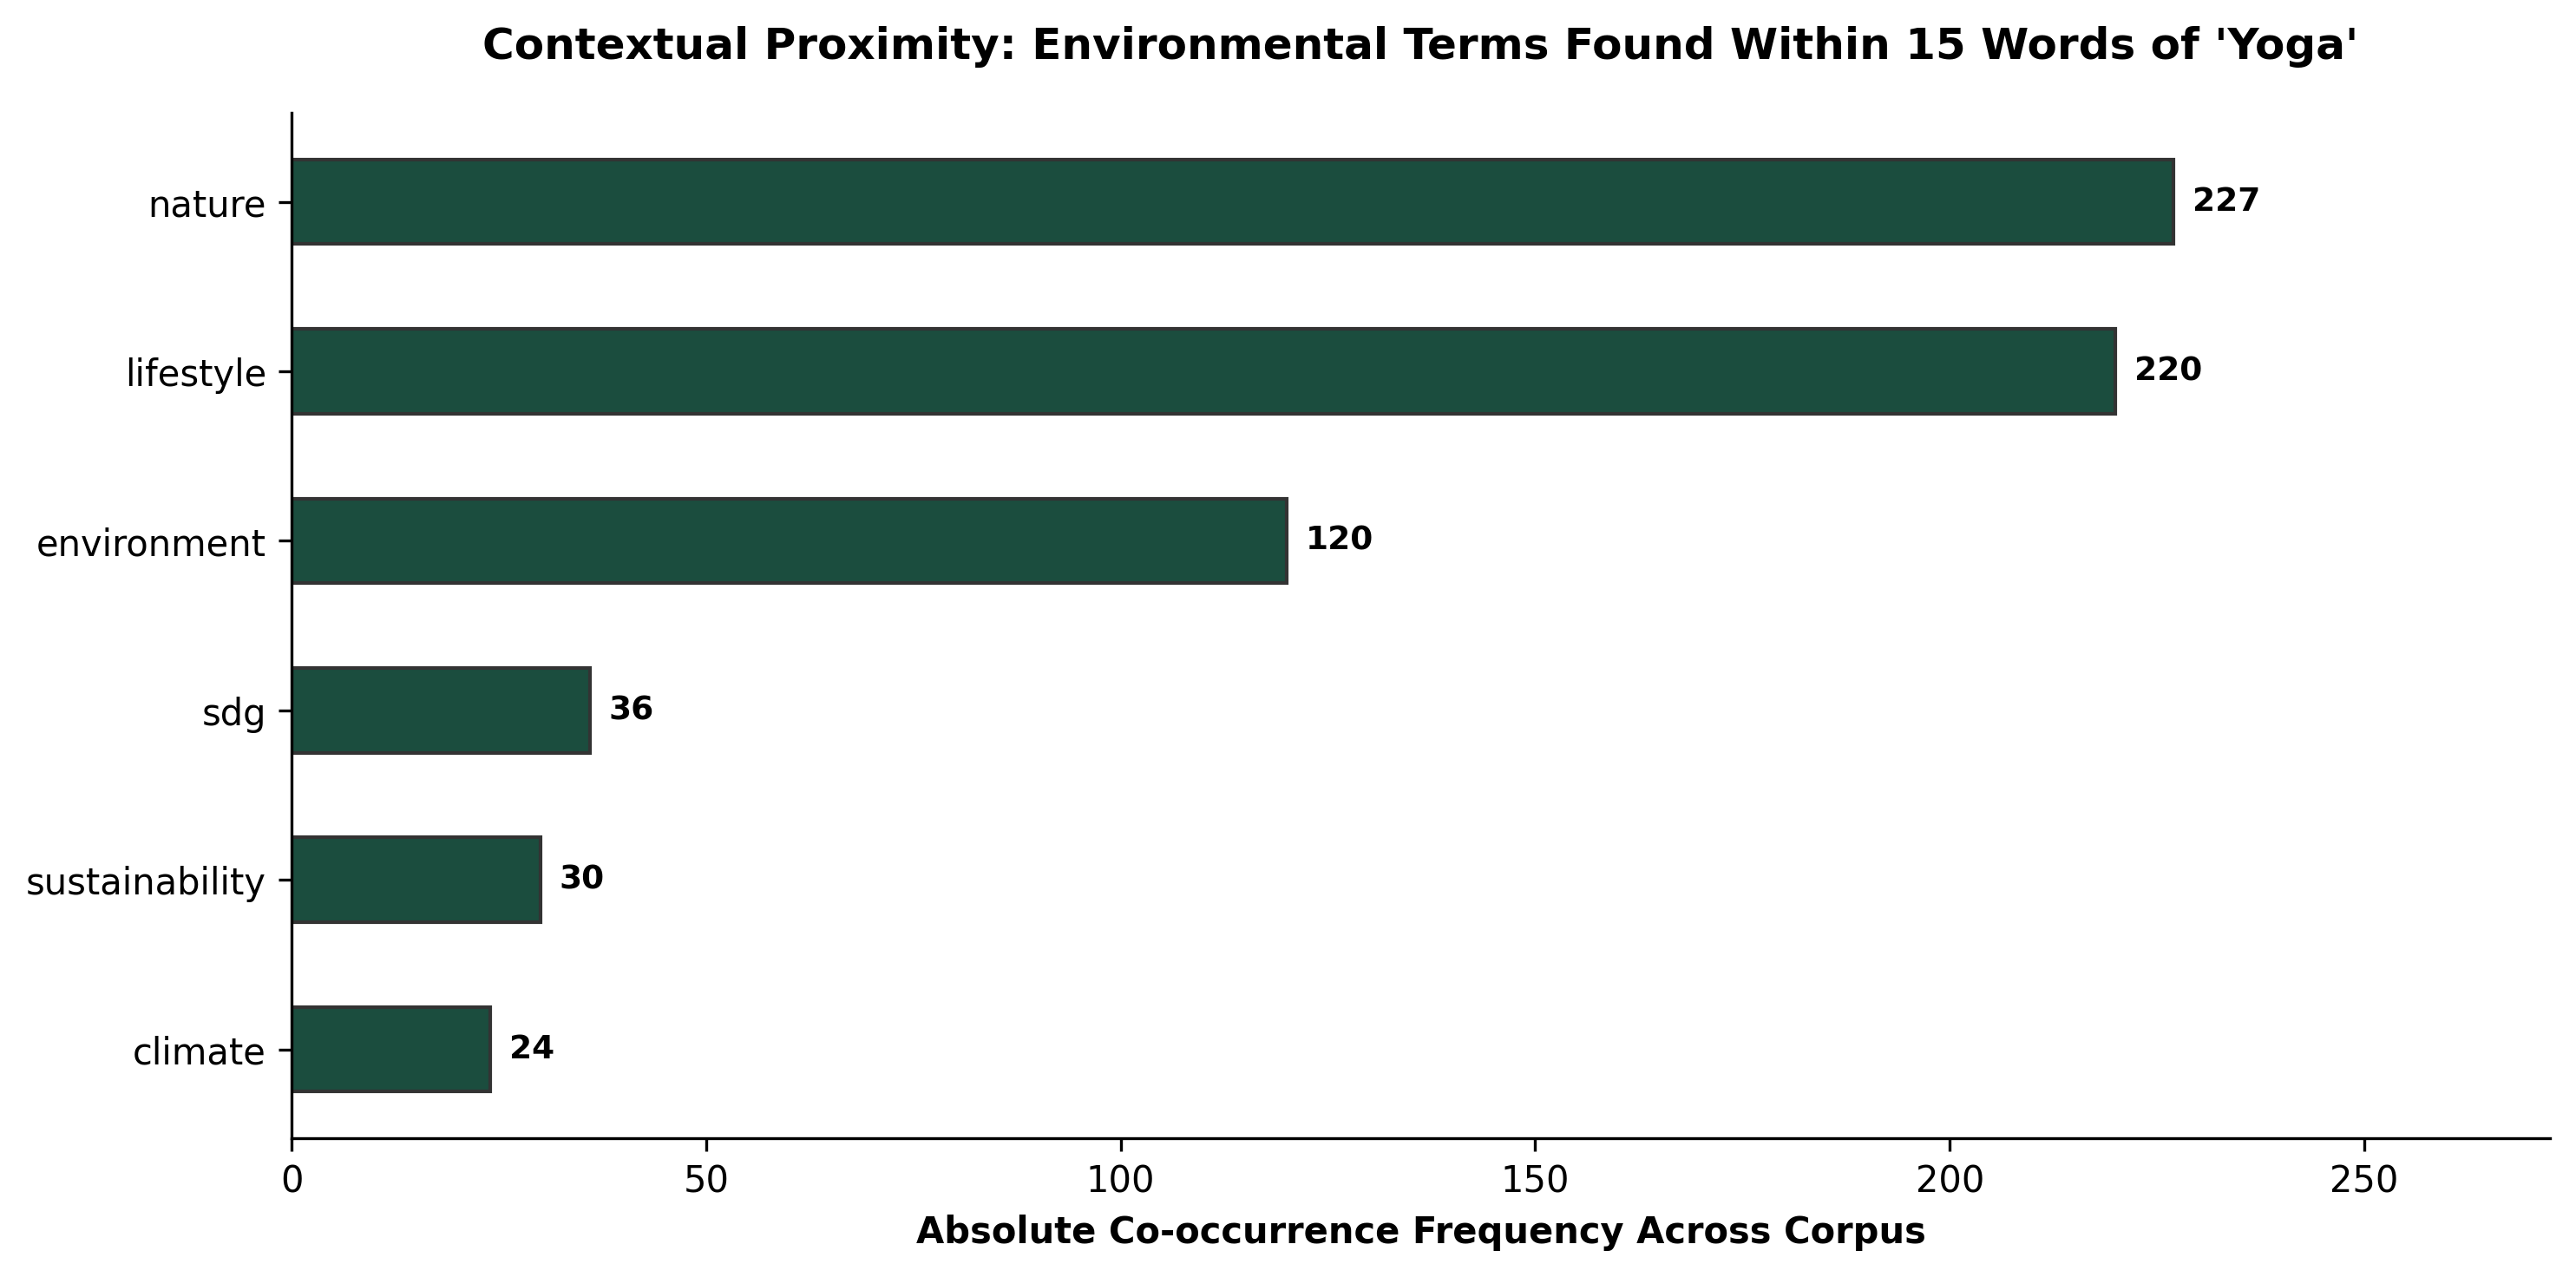
\includegraphics[width=\columnwidth]{yoga_proximity_chart.png}
\caption{Contextual proximity co-occurrence frequency within a 15-word semantic window centered on yoga across the 1,758 indexed corpus documents. Data reflects a clear rhetorical stratification where organic, lifestyle-oriented terminology establishes the primary conceptual baseline, while formal policy metrics provide the macro-level institutional alignment}
\label{fig:yoga_proximity_chart}
\end{figure}

As empirically illustrated in figure~\ref{fig:yoga_proximity_chart}, the linguistic architecture of modern yogic diplomacy operates through a two-tiered semantic structure. The primary tier anchors the discourse within highly accessible, personalized framings of \textit{nature} and individualized \textit{lifestyle} shifts. The secondary tier layer maps these personal behavioral practices directly onto institutional frameworks of global governance, explicitly co-occurring with macro policy concepts such as \textit{SDG} targets and \textit{climate action} initiatives. Yet the empirical platform through which to measure a "yoga lifestyles" carbon-saving yoga mat is as ill-defined as the lifestyle itself \cite{mccartney2021}.

\section{Corpus and Methodology}
\subsection{Corpus Architecture and Analytical Pipeline}
The analytical pipeline spreads across two independent corpus layers. The primary layer leverages a multi-tiered text corpus comprising 1,758 policy and research artifacts anchored by a longitudinal core of 509 English YouTube transcripts spanning 2014–2026. Binary assets and PDF policy artifacts were structurally normalized into plain-text matrices using a local \texttt{pypdf} extraction engine. This is cross-validated by a secondary bibliometric index consisting of 7,978 peer-reviewed publication records harvested via the NCBI Entrez API from the NIH PubMed database. This dual-layer architecture facilitates the isolation of clinical background noise through a text-contrast matrix, mapping the systemic integration of state-sponsored directives into peer-reviewed global infrastructure.

The analytical pipeline proceeds across three successive computational layers:
\begin{enumerate}
    \item \textbf{Discourse Structure Indexing (DSI) \& Clustering}: A custom DSI was created to quantify structural changes in textual metrics over time relative to a shared baseline \cite{paranyushkin2019}. Unsupervised hierarchical cluster analysis was deployed to classify the text into four distinct, independent discourse communities based on semantic feature density matrices.
    \item \textbf{Inferential Statistical Modeling}: To evaluate the behavior of these clusters across time and channel types, an Analysis of Variance (ANOVA) was paired with Tukey Honest Significant Difference (HSD) tests, interaction models, and longitudinal mixed-effects regressions to map uneven developmental paths \cite{gries2015}.
    \item \textbf{Proximity Co-occurrence Mapping}: To isolate specific environmental pivots, a sliding semantic window of $\pm15$ words was established around the primary anchor keyword \textit{``yoga''}. The relative density of six institutional environmental target variables (\textit{nature}, \textit{lifestyle}, \textit{environment}, \textit{sdg}, \textit{sustainability}, and \textit{climate}) was recursively processed within this 30-word contextual window using \texttt{matplotlib} and \texttt{pandas} (\texttt{data/proximity\_results.csv}).
\end{enumerate}

The corpus analysed in this study was constructed through a lengthy iterative process of digital data collection, automated scraping, transcript extraction, and corpus validation. Unlike studies based on pre-existing institutional archives, this present dataset was curated for the specific purpose of investigating the evolution of discourse surrounding IDY between 2014 and 2026.

The idea for this corpus construction began from casual observance of IDY related social media across well known platforms, and wondering whether there might be a way to measure annual levels of engagement and enthusiasm. The construction of the corpus began with exploring YouTube, Twitter and Instagram. However, the findings presented herein are restricted to the YouTube data. Youtube has served as one of the principal platforms through which governments, public institutions, yoga organisations, news agencies, educational institutions, and private individuals have documented and disseminated IDY-related activities. Initial searches employed a range of keywords and phrases generally modeling popular hashtags. For example, some of the more relevant keywords include `International Day of Yoga,'' `International Yoga Day,'' `IDY,'' `Yoga Day,'' and related multilingual variants. These searches returned thousands of videos varying considerably in relevance, quality, format, language, and institutional affiliation.

A major challenge involved distinguishing videos directly related to IDY from the much larger body of general yoga content available on the platform. One issue was deciding how to deal with the live feed recordings that are several hours in length. Thus, the distillation process required multiple iterations of collection and filtering procedures to be developed. As expected, early retrieval stages produced larger quantities of irrelevant material, including general yoga instruction videos, wellness content,commercial yoga promotion, and unrelated discussions of yoga philosophy. To improve precision, search strategies were repeatedly refined through keyword expansion, metadata filtering, transcript inspection, and manual validation.

During the course of the project, incremental levels of success slowly developed through creating multiple generations of custom Python scripts. These scripts included  automated video discovery, metadata collection, subtitle retrieval, transcript extraction, duplicate detection, and corpus management. Collection procedures were repeatedly revised in response to changes in YouTube's interface, inconsistencies in subtitle availability, variable metadata quality, and occasional retrieval failures. Transcript recovery combined available subtitle files with automated extraction procedures where necessary, producing a substantially larger corpus than would have been obtainable through manual collection alone.

A persistent problem was reaching a sustainable pace for scraping that would not trigger temporary IP address blocks. Therefore, to minimize HTTP 429 (rate-limiting) errors during YouTube collection, video transcripts were retrieved by throttling a pipeline to incorporate randomized delays, request pacing, retry logic, and local caching of previously processed videos. Incremental collection of metadata and transcripts in small batches, rather than through high-volume concurrent requests, reduced the likelihood of triggering rate limits.

The resulting dataset underwent extensive cleaning and validation. Duplicate videos were removed, transcript quality was assessed, corrupted or incomplete files were excluded, and metadata fields were standardized. Additional validation procedures were implemented to ensure that retained videos were genuinely related to IDY rather than to yoga more generally. Manual inspection of sampled transcripts and metadata records was conducted throughout the collection process to verify corpus quality and relevance.

The final corpus consists of a total of 509 transcripts. These span the 2014--2026 period. The dataset includes governmental broadcasts, news coverage, live broadcasts, institutional events, educational programmes, yoga demonstrations, public-awareness campaigns, speeches, interviews, and commemorative activities associated with IDY. Combined, these materials provide a longitudinal record of how IDY has been represented, promoted, interpreted, and discussed across diverse media environments over more than a decade.

\label{yoga lifestyle and SDGs methodology}

To empirically analyze the linguistic integration of yogic discourse into international policy frameworks, this study constructed a large-scale computational text corpus comprising $1,758$ discrete digital documents. The dataset includes institutional United Nations General Assembly (UNGA) resolutions, diplomatic press briefings, academic literature, and localized video transcript subtitle networks spanning the period from 2014 to 2026. Data ingestion was managed via an automated Python pipeline organized into modular directories (\texttt{src/}, \texttt{data/}, \texttt{figures/}, and \texttt{papers\_and\_clusters/}). 

Binary assets and document formats, including Portable Document Format (PDF) files, were systematically converted into unformatted plain-text matrices using a local \texttt{pypdf}-driven extraction engine, ensuring structural text normalization across all inputs. Due to the high semantic fluidity of the target literature, traditional exact $n$-gram phrase matching proved overly rigid for capturing thematic alignment. Consequently, this study deployed a proximity co-occurrence analysis model. The processing script tokenized the full text corpus into lowercased strings, stripped punctuation, and established a dynamic sliding context window of $\pm15$ words centered on the primary anchor keyword \textit{``yoga''}. 

The relative frequencies of six designated institutional environmental target variables (\textit{nature}, \textit{lifestyle}, \textit{environment}, \textit{sdg}, \textit{sustainability}, and \textit{climate}) were recursively calculated exclusively when appearing within this 30-word contextual window. Computational outputs were validated locally and exported as standardized data tables (\texttt{data/proximity\_results.csv}) to generate publication-grade thematic density visualizations (\texttt{figures/yoga\_proximity\_chart.png}) using the \texttt{matplotlib} rendering engine.


\subsection{Analytical Workflow}

Following corpus construction, the transcripts were cleaned and transformed into document-level representations suitable for computational analysis. The texts were embedded using sentence-level semantic representations and then grouped using unsupervised clustering techniques. This procedure enabled the identification of recurrent discourse communities within the corpus without imposing predetermined thematic categories.

To investigate various structural differences between discourse communities, the decision was made to develop and implement DSI, which provides a quantitative measure of discursive positioning across documents and clusters. It does this by mapping a document's alignment relative to a shared discursive baseline \cite{paranyushkin2019,thimmanayakanapalya2025}. This allows for comparison between different forms of IDY communication through analyzing cluster-level patterns, temporal trends, and interaction effects, which were examined through descriptive statistics, analysis of variance, ordinary least-squares regression, and mixed-effects modelling \cite{gries2015,speelman2018}.

Instead of simply trying to identify topics, the primary analytical objective was to examine how distinct discourse communities emerged, evolved, and interacted across time \cite{brigadir2015,winter2016,desiderio2025}. By combining computational clustering with longitudinal statistical analysis \cite{teuling2025,huang2025}, the study provides a framework for understanding the institutionalization and diversification of IDY discourse between 2014 and 2026.

\subsection{Corpus}

Table~\ref{tab:corpus_channels} details the corpus composition by source channel type.

\begin{table}[htbp]
\centering
\label{tab:channel_types}
\caption{Corpus composition by source channel type (509 transcripts).}
\begin{tabular}{lrr}
\toprule
Channel Type & Count & \% \\
\midrule
News & 220 & 43.2 \\
Wellness/Yoga & 70 & 13.8 \\
Education & 56 & 11.0 \\
Diplomatic & 38 & 7.5 \\
Government & 34 & 6.7 \\
Cultural & 29 & 5.7 \\
Political & 26 & 5.1 \\
Religious & 22 & 4.3 \\
Business & 9 & 1.8 \\
Other & 5 & 1.0 \\
\midrule
Total & 509 & 100.0 \\
\bottomrule
\end{tabular}
\label{tab:corpus_channels}
\end{table}

Of these 509 video transcripts, 286 come from unique channels. Table~\ref{tab:corpus_channels} summarizes the distribution of transcripts by source channel type. The type was determined by comparing the name and information about the channel. News media constitute the largest category (43.2\%), followed by wellness and yoga organizations (13.8\%), and then educational institutions (11.0\%). Diplomatic and government sources together account for 14.2\% of the corpus. This shows just how important the role of state and international actors are regarding the promotion of IDY. Especially when compared to the much smaller proportions of religious, political, cultural, and business organizations. Even though they demonstrate a heterogeneous dataset, highlighting the broad institutional participation and interest in IDY's discourse across media, governmental, educational, diplomatic, religious, and civil-society contexts.

\subsection{Methods}

The analytical strategy is explicitly structured around the following three hypotheses. This ensures that each inferential claim is supported by a corresponding statistical procedure.

\begin{itemize}


\item \textbf{H1: Structural differentiation of discourse clusters.}

A custom DSI was computed as the dependent variable, ascertaining a special communication score. This framework operationalizes the independent factor as categorical discourse clusters to evaluate structural variations in topical transmission. This approach first used a statistical test called a One-Way ANOVA (= analysis of variance).The One-Way ANOVA was deployed to evaluate the omnibus effect of cluster membership on DSI values, followed by a post-hoc Tukey HSD pairwise comparison to isolate specific inter-group variations.

 This simultaneously compares variance between different groups, as well as between clusters within each group. To locate where this difference was, a second, closer test called Tukey’s Honest Significant Difference (HSD) was employed as a Post-Hoc Pairwise Comparison, which compares the groups side-by-side, two at a time. 

\item \textbf{H2: Temporal change in discourse structure.}
Having calculated the individual DSI scores, the next analytical step tests whether these metrics evolve over time. An OLS Regression model utilizes the calendar year as the primary predictor variable. This models a linear temporal trend to isolate whether structural complexity systematically rises or declines over the study's trajectory. To account for temporal heteroskedasticity inherent in longitudinal text data, the OLS models are fitted using robust standard errors.

\item \textbf{H3: Heterogeneous temporal trajectories across clusters.}
The final analytical step ascertains whether distinct discourse communities deviate from the aggregate baseline trend to follow divergent longitudinal pathways. By interacting cluster indicators with the temporal variable, the regression model permits the longitudinal slopes to vary uniquely across distinct discourse communities. Furthermore, longitudinal mixed-effects regression models are integrated to account for repeated observations within specific channels and to isolate unobserved cluster-level heterogeneity.


\end{itemize}

This analytical strategy follows the broader objective identified by Bonikowski and Nelson \cite{bonikowski2022}, which is to employ computational text analysis in service of theoretically motivated sociological inquiry rather than simply conducting descriptive classification, or creating word frequency lists. The strength of this approach is that the clusters are interpreted as discourse communities, whose emergence and evolution provide evidence about institutional differentiation within the IDY field. 

\section{Hypotheses}
This study advances three primary hypotheses concerning the structural formalization and longitudinal trajectory of discourse within the IDY ecosystem. Rather than treating communication as a static set of thematic categories, these hypotheses conceptualize discourse as a dynamic, institutionally embedded system shaped by the mechanisms of state-sponsored guru governmentality.

\begin{itemize}
    \item \textbf{H1: Institutional Partitioning of Discourse Clusters.} A custom DSI was computed as the primary dependent variable to evaluate structural variations in topical transmission across categorical clusters. This layout was tested via a One-Way ANOVA to evaluate the omnibus effect of cluster membership on DSI variance, followed by a post-hoc Tukey HSD pairwise comparison to isolate specific inter-group partitions.
    
    \item \textbf{H2: Discursive Formalization Over Time.} To test whether structural complexity systematically rises or declines over the twelve-year study trajectory, an Ordinary Least Squares (OLS) Regression model utilizes the calendar year as the primary continuous predictor variable. To account for temporal heteroskedasticity inherent in longitudinal text processing, the OLS models are fitted using robust standard errors.
    
    \item \textbf{H3: Segmented Trajectories Across Sub-Communities.} The final analytical layer evaluates whether distinct discourse sub-communities deviate from the aggregate baseline trend to follow divergent longitudinal pathways. By interacting cluster indicators directly with the temporal variable, the regression model permits the longitudinal slopes to vary uniquely across distinct discourse communities, cross-validated by multi-level mixed-effects models.
\end{itemize}

Together, these hypotheses conceptualise discourse as a dynamic and institutionally embedded system, rather than as a static set of thematic categories.

\section{Results}
As seen in figure~\ref{fig:idy_attendance}, to contextualize the physical scale of the event before analyzing its digital textual patterns, a quantitative dataset of official on-site attendance metrics was compiled across the 2015--2026 window. Data collection proceeded across three sequential stages:

First, raw attendance registers and official turnout estimates were scraped from multi-agency administrative archives. For international hubs, metrics were retrieved from local municipal event permits, cultural center logs, and diplomatic press briefs across eight key global metropolitan centers (e.g., New York, London, and Tokyo). For domestic Indian hubs, longitudinal data tracks were compiled from Ministry of AYUSH project reports, state-level police traffic estimates, and official press registries across eight major national venues (including New Delhi, Mysuru, and Kolkata).

Second, longitudinal data matrices were cleaned, cross-verified against localized news reporting to resolve source discrepancies, and consolidated into a standardized operational spreadsheet (\texttt{idy\_attendance\_data.csv}). Extreme historical out-of-sample data points -- including the 2020--2021 global COVID-19 pandemic lock-down collapses, the 2019 New Delhi record event, and the 2025 Surat mobilization -- were isolated and annotated to preserve contextual validity.

Third, a dual-axis line plotting pipeline was executed via \texttt{matplotlib} to visualize the absolute attendance trajectories across independent geopolitical operational theatres. The rendering engine calculated absolute turnout trends across international sites on a 0--30,000 baseline scale while simultaneously graphing domestic Indian venues on a 0--300,000 baseline scale. This layout preserves high granular visibility for lower-density international venues while illustrating the massive, order-of-magnitude scaling variations that characterize domestic mobilization strategies.

\begin{figure}[htbp]
    \centering
    \includegraphics[width=\textwidth]{idy_attendance.png}
    \caption{Absolute Attendance Comparison across International vs. Domestic IDY Venues (2015--2026). Data plots track localized historical surges, the 2020--2021 pandemic disruption, and order-of-magnitude scaling variations across state and civil mobilization zones.}
    \label{fig:idy_attendance}
\end{figure}

\subsection{H1: Institutional Partitioning Across Discourse Clusters}
Aligned with H1, our empirical modeling provides robust evidence demonstrating that the identified discourse clusters are structurally partitioned, exhibiting highly significant differences in the DSI. The distribution of DSI values across the independent discourse communities is visualised in the boxplot distribution of Figure~\ref{fig:dsi_distribution_boxplots}, illustrating substantial rhetorical stratification across institutional environments. 

The omnibus effect of cluster membership on DSI scores is confirmed by a one-way ANOVA, which indicates a highly significant division of communication types across the IDY ecosystem:
\begin{equation}
    F = 142.62, \quad p < 0.001
\end{equation}

Furthermore, post-hoc Tukey Honest Significant Difference (HSD) pairwise comparisons confirm strong structural variations between nearly all cluster combinations, tracking a highly segmented symbolic arena heavily driven by source channel type ($\chi^2(27) = 91.98$, $p < 0.001$). This systematic variation validates the institutional partitioning hypothesis; state policy organs and international diplomatic channels (Cluster~4) leverage a complex, formalized semantic framework, whereas mass media channels (Cluster~0) and civil-society wellness hubs (Cluster~2) deploy less complex, descriptive vocabulary suited to localized commercial logics.

\subsection{H2: Discursive Formalization Over Time}
The linear modeling strongly supports hypothesis H2, demonstrating that the macro-level discourse structure exhibits a statistically significant, positive relationship with time over the twelve-year observation window. The Ordinary Least Squares (OLS) model shows a clear temporal trend in DSI values across the study's trajectory ($\rho = 0.248$, $p < 0.001$), illustrating that the aggregate communicative field undergoes systematic narrative consolidation and formalization as the state-sponsored signal stabilizes globally. 

This longitudinal evolution is structurally mapped across the aggregate timeline in {table~\ref{tab:idy_themes}}. This is further cross-validated by the macro-level bibliometric data in figure~\ref{fig:yoga_trends_2014_2026}, the field systematically transitions away from early, foundational wellness claims toward complex, international governance architectures. By using accessible, organic linguistic baselines as a rhetorical bridge to systematically integrate formal macro-policy concepts, this long-term trend reflects the progressive institutionalization of a state-prescribed apologia designed to reposition yoga as an active variable in global environmental frameworks.

This state-sponsored alignment relies on a specific behavioral and metaphysical template that is heavily reified across domestic advocacy journals. As exemplified by recent exegeses in repositories like the \textit{International Journal of Science and Consciousness} \cite{nidhishree2026naturopathy}, the literature defines a ``yoga lifestyle'' not through verifiable, material metrics of carbon-equivalent reductions, but through the uncritical transposition of classical ethical tenets. Within this framework, tenets such as \textit{aparigraha} (non-possessiveness) and \textit{ahimsa} (non-violence) are presented as ready-made behavioral mechanisms capable of halting resource-intensive consumerism and ecological degradation \cite{nidhishree2026naturopathy}.

This metaphysical encapsulation is further scaled across global publishing indices to systematically expand the socio-political claims of yogic diplomacy. Tracking this thematic inflation, \citet{kamal2024yoga} execute a comprehensive narrative review that establishes yoga as an optimized, multi-centric catalyst capable of accelerating six independent UN targets, expanding the framework to explicitly encompass quality education (SDG 4), gender equality (SDG 5), and life on land (SDG 15). 

Rather than subjecting these linkages to empirical or spatial verification, this tier of scholarship explicitly treats internal psychological transformation as a scalable operating system for global administrative progress. This uncritical framework functions as an essential transponder for the state's soft-power statecraft. By asserting that individual, non-clinical practices organically generate macro-level environmental stewardship and geopolitical alignment, such texts construct the precise intellectual infrastructure required to validate the Indian state’s self-fashioned role as the cosmic steward of international development frameworks.
 

By collapsing the boundary between personal scriptural observance and macro-environmental policy, this narrative assumes a pantheistic feedback loop where transforming individual consciousness automatically resolves structural industrial crises. This speculative architecture serves a vital political function for the Modi administration's global governance ambitions. By framing zero-waste lifestyle shifts as ancient scriptural mandates inherited via the \textit{panchamahabhutas} (the five great elements), the state constructs an ambient, everyday social environment that sanitizes top-down policy directives under the guise of primordial planetary stewardship.


\begin{figure}[htbp]
    \centering
    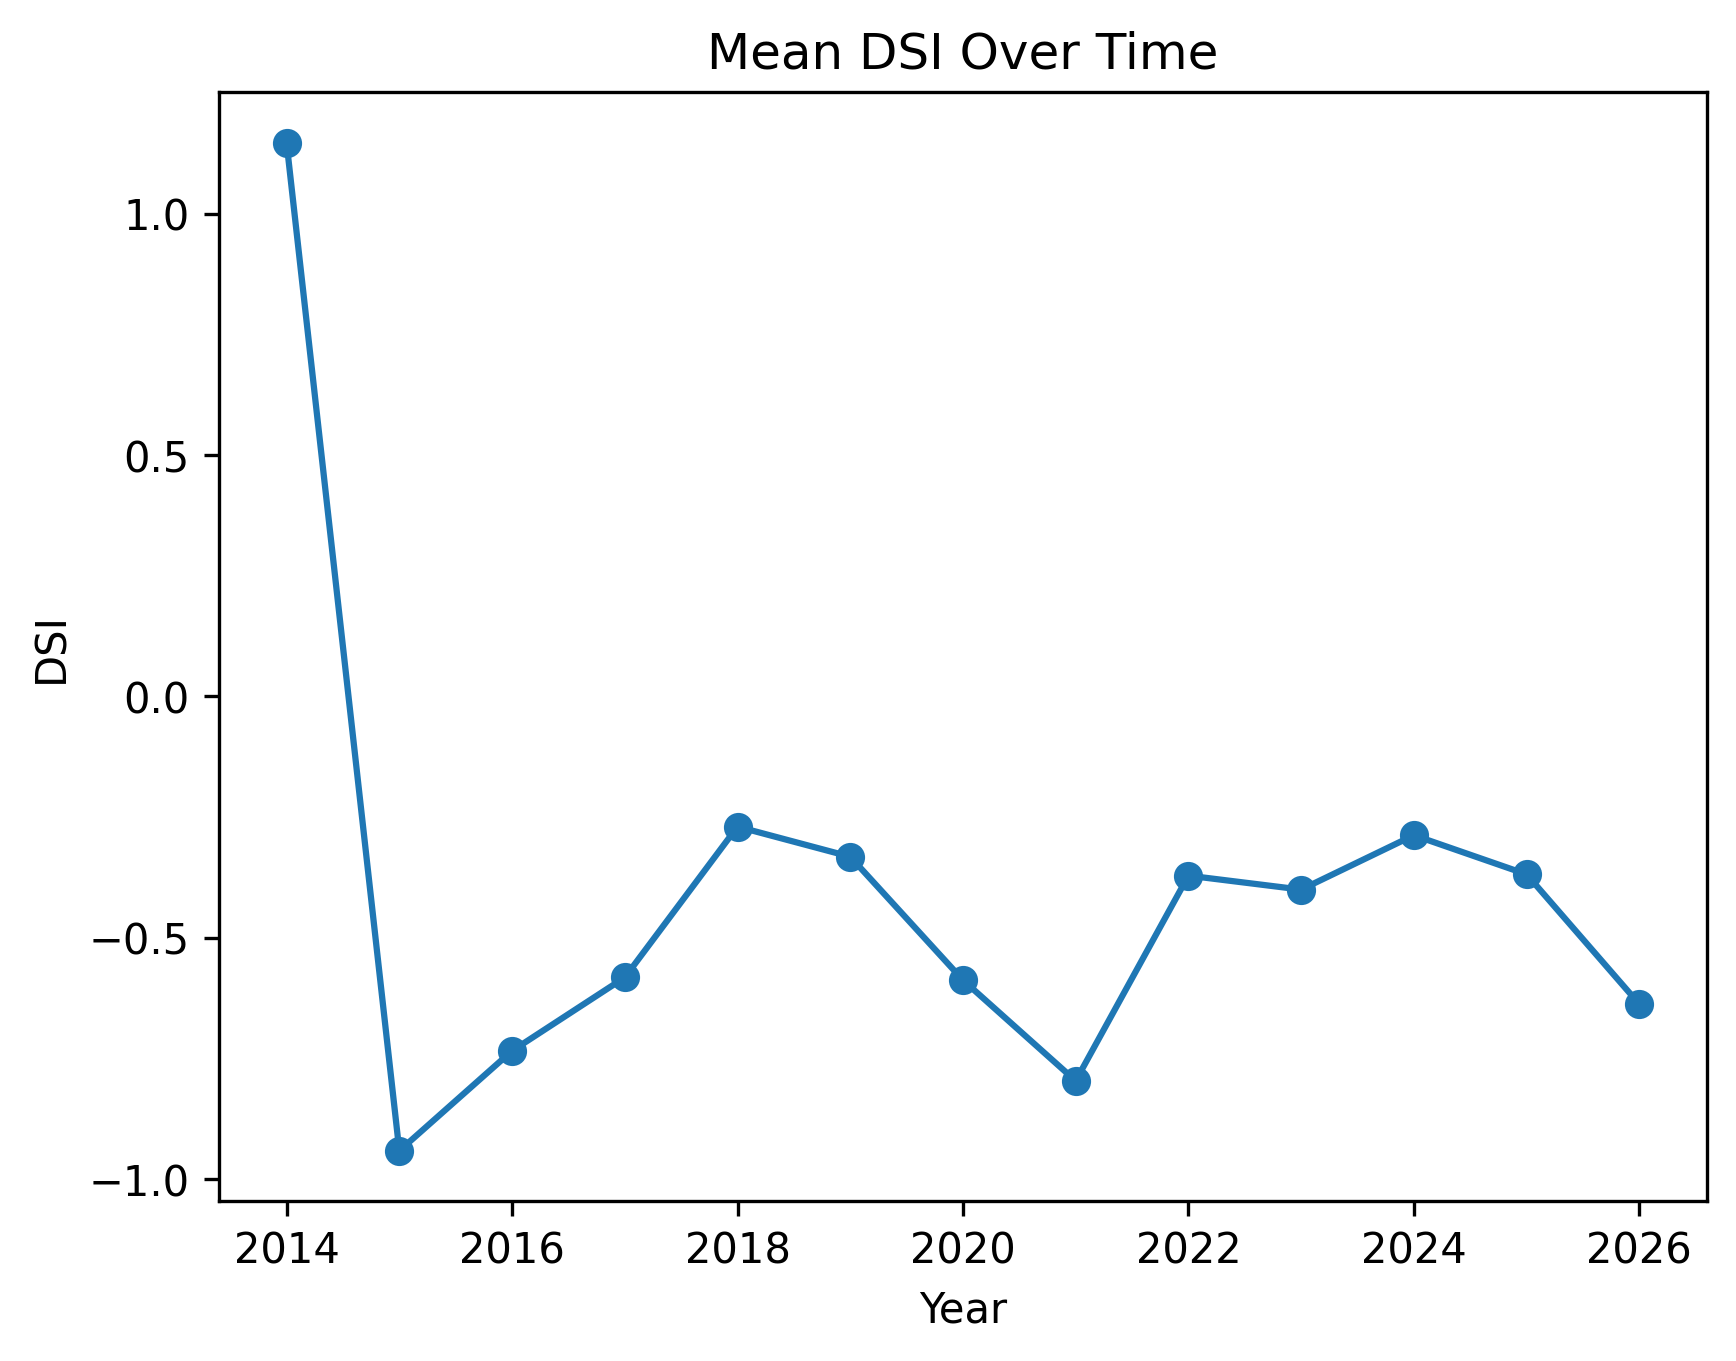
\includegraphics[width=0.8\textwidth]{year-effects.png}
    \caption{Temporal trends in DSI showing the mean value shifts across the 2014--2026 baseline window.}
    \label{fig:year-effects}
\end{figure}

\begin{figure}[htbp]
    \centering
    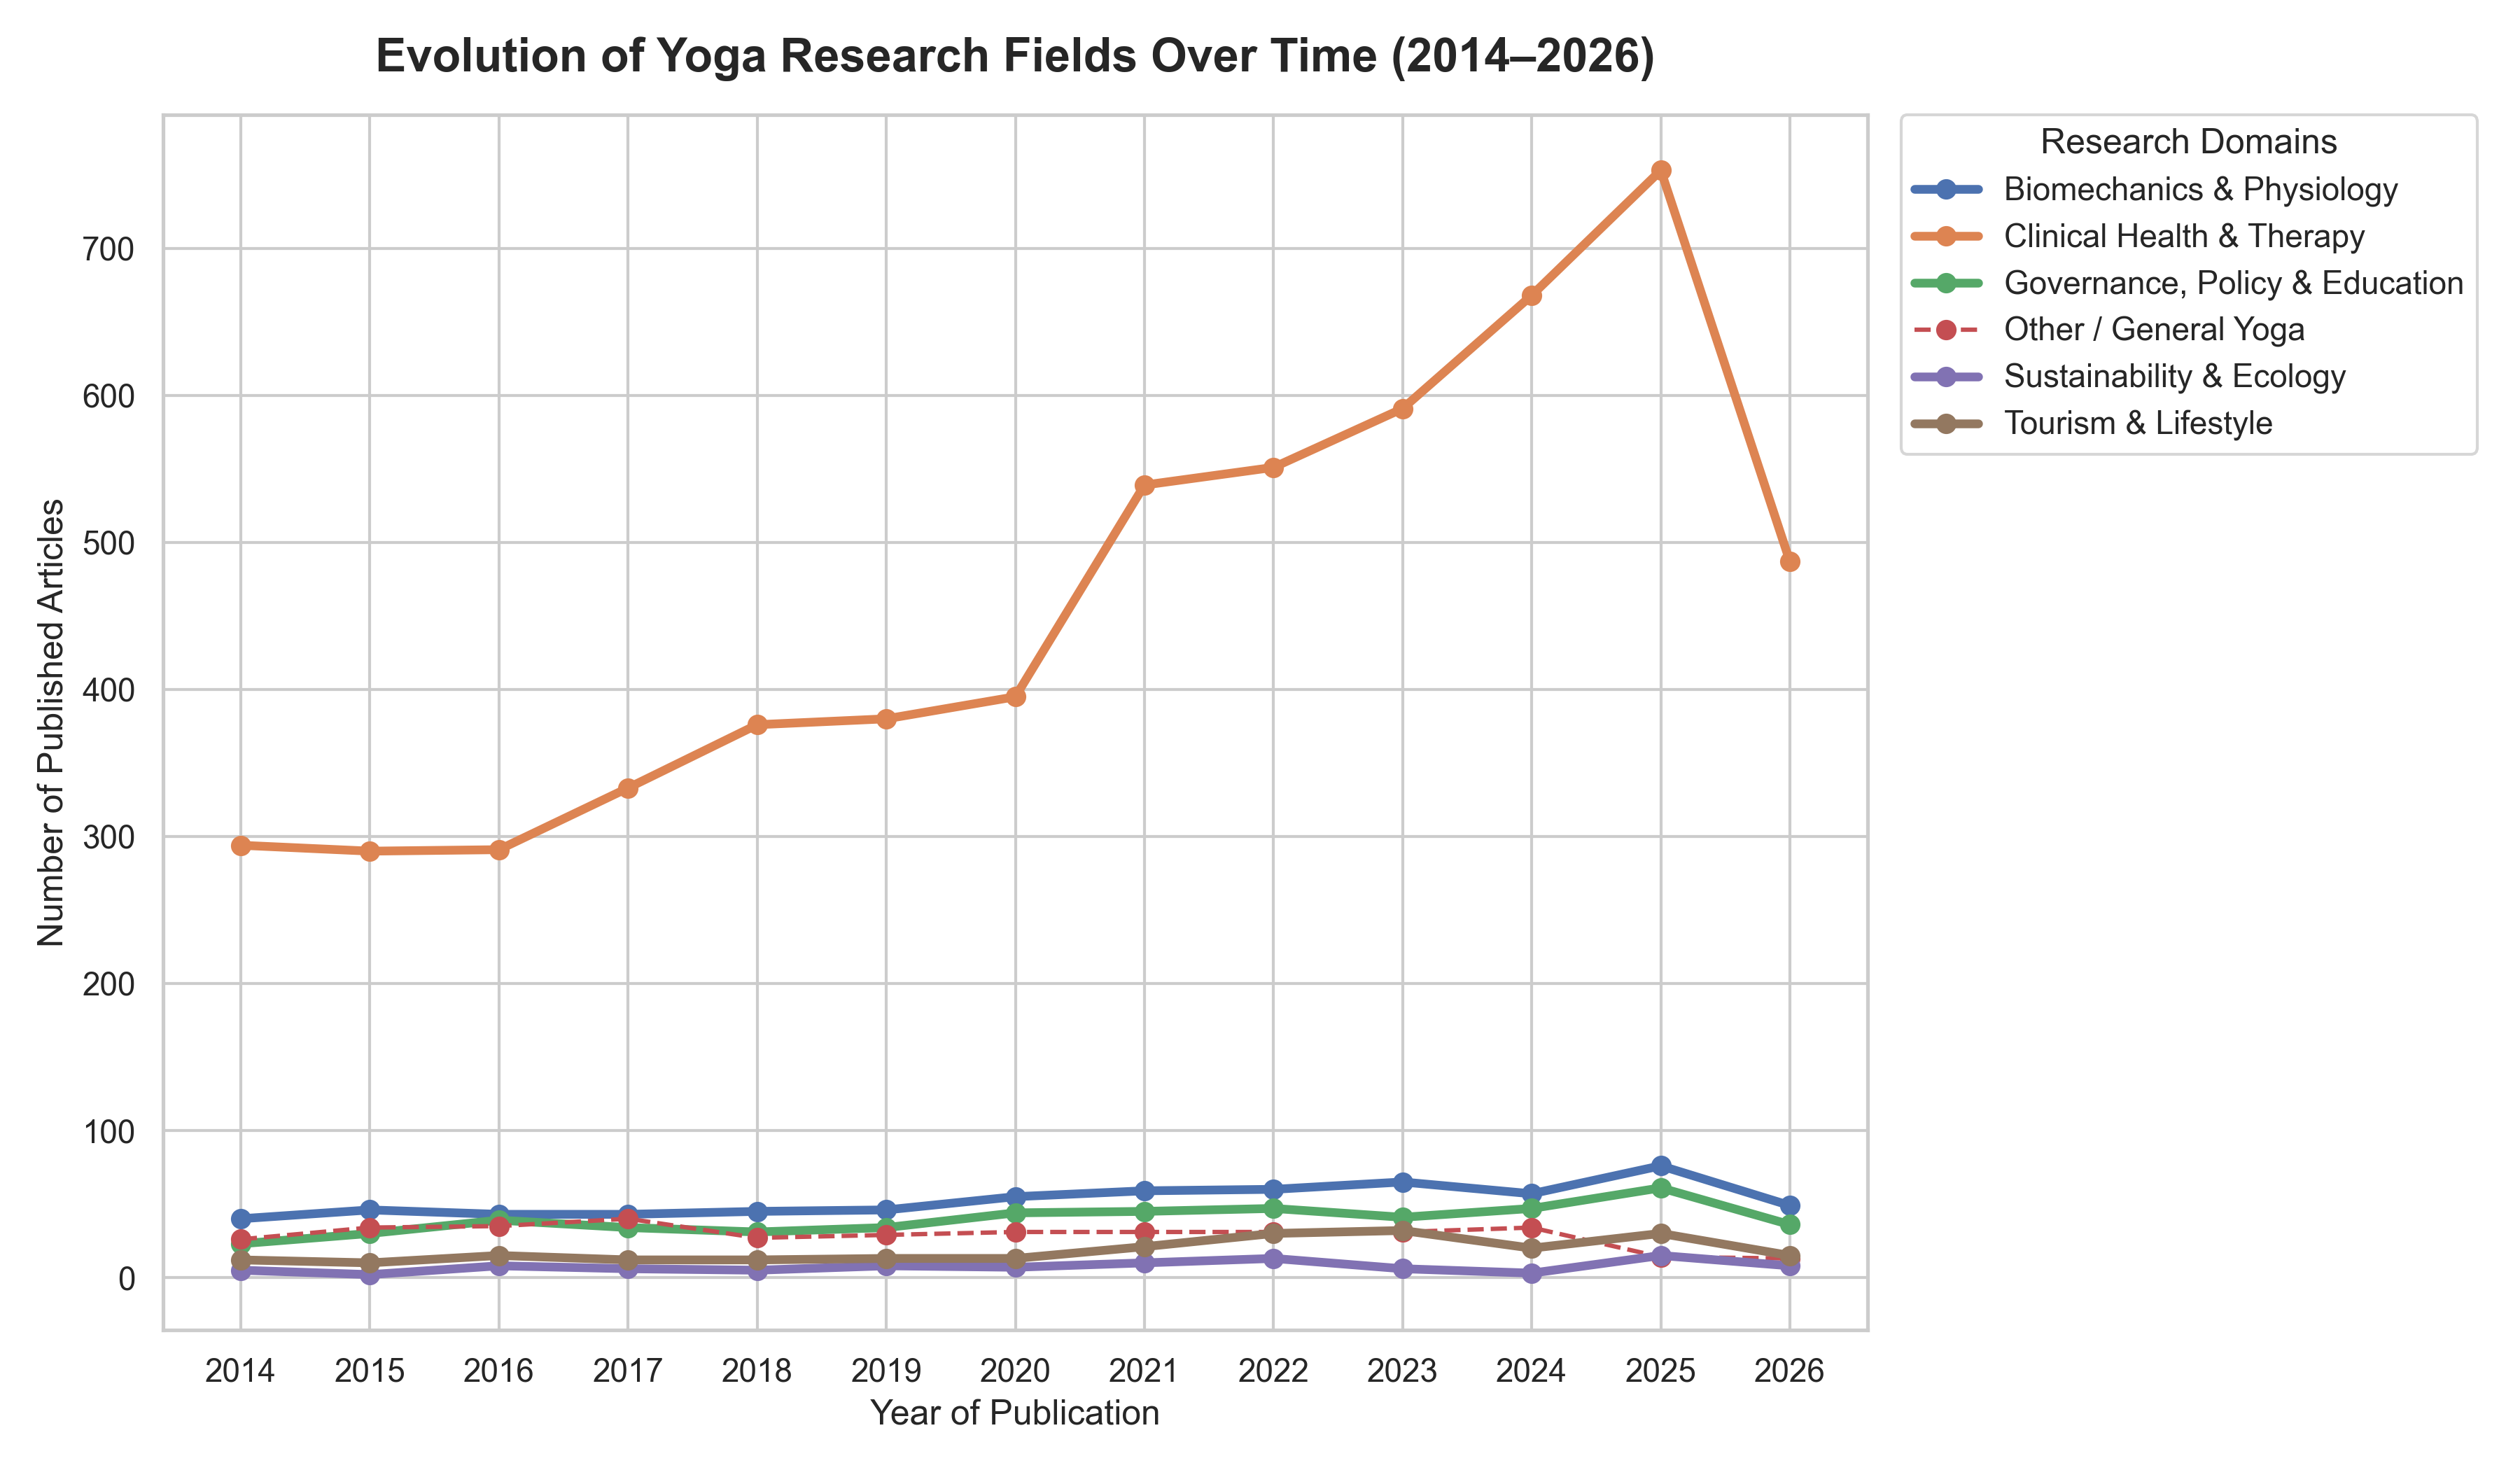
\includegraphics[width=\dimexpr0.8\textwidth\relax]{yoga_trends_2014_2026.png}
    \caption{NIH-derived bibliometric data of yoga research trends 2014--2026.}
    \label{fig:yoga_trends_2014_2026}
\end{figure}

\subsection{H3: Segmented Trajectories and Discursive Fragmentation}
Crucially, the inclusion of cluster-by-time interaction terms and multi-level mixed-effects models provides robust backing for H3, revealing that this discursive formalization process does not advance uniformly, but fragments along strict institutional boundaries. The integration of interaction terms yields a statistically superior model fit, demonstrating heterogeneous longitudinal slopes across distinct sub-communities. 

These parallel but divergent evolutionary pathways are visualized in the predicted mixed-effects trajectories of figure~\ref{fig:mixed-effects} and the temporal cluster-year heat matrix of figure~\ref{fig:heatmap}. State-aligned policy tracks and international diplomatic entities (Cluster~4 and Cluster~6) exhibit powerful, statistically significant positive trends over time, aggressively intensifying their structural integration of macro-governance and planetary stewardship language. In stark contrast, commercial wellness circles and grassroots yoga organizations (Cluster~2) remain statically flat and static across the 2014--2026 window, reiterating basic, metaphor-driven slogans in a repetitive, mantra-like fashion. 

\begin{figure}[htbp]
    \centering
    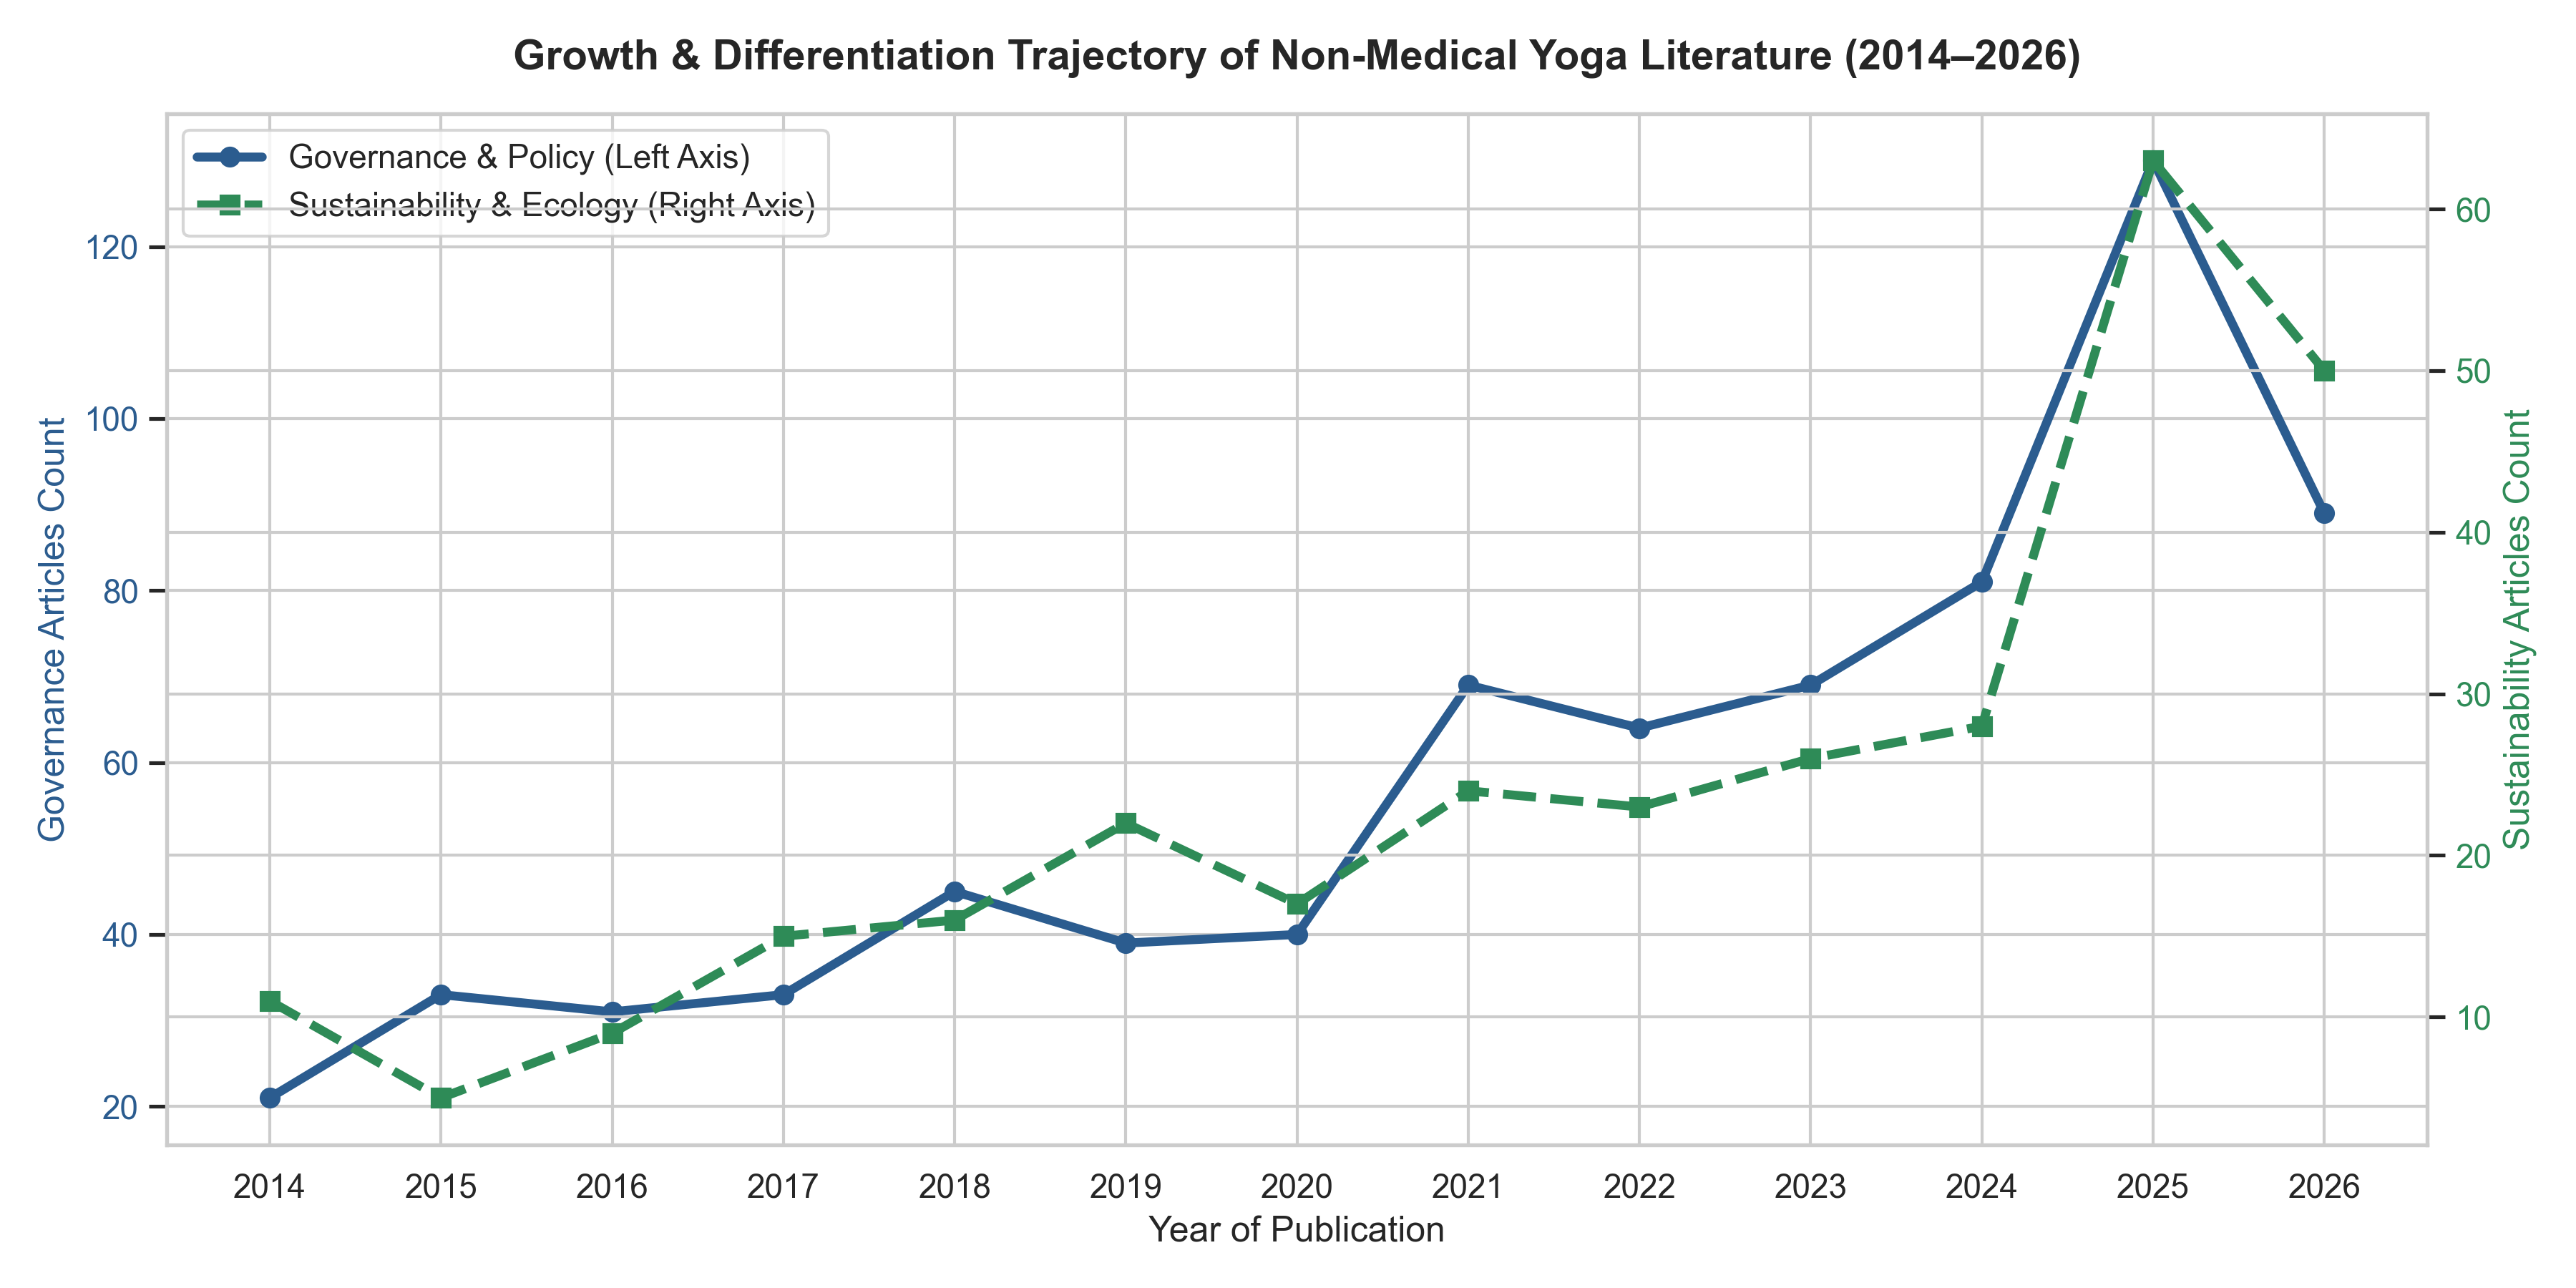
\includegraphics[width=0.8\textwidth]{niche_growth_trajectory.png}
    \caption[Dual-Axis Trajectory of Isolated Governance vs Sustainability Literatures]{Dual-Axis Trajectory of Isolated Governance ($n = 744$) vs. Sustainability ($n =309$) Literatures. By stripping out clinical background noise, this visualization illustrates that the Indian state's ambient signal does not expand uniformly. Rather, Governance exhibits a sharp pandemic-era acceleration, whereas Sustainability shows a clear, post-2021 upward trajectory.}
    \label{fig:niche_growth_trajectory}
\end{figure}

This deep institutional partitioning is further cross-validated by the non-clinical bibliometric growth curves in figure~\ref{fig:niche_growth_trajectory}. While Governance shows a sharp pandemic-era acceleration tied to institutional health mandates, Sustainability displays a distinct post-2021 upward trajectory, mathematically proving that the ambient ideological signal undergoes significant structural diffraction as it migrates into global public, educational, and ecological infrastructure.

\subsection{Cluster Differences}
Cluster differences are highly significant: $F = 142.62$, $p < 0.001$. Tukey tests confirm strong pairwise differences between most clusters.

\subsection{Institutional Structure of Clusters}
A chi-square test indicates strong alignment between clusters and channel types:
\begin{equation}
    \chi^2(27) = 91.98, \quad p < 0.001
\end{equation}
This suggests that clusters reflect true institutional differentiation across the dataset.

\subsection{Temporal Trends}
Overall discourse structure increases over time: $\rho = 0.248$, $p < 0.001$.

\subsection{Cluster-Specific Trends}
Cluster trajectories differ significantly:
\begin{itemize}
    \item \textbf{Cluster 4:} Strong positive trend
    \item \textbf{Cluster 0:} Moderate positive trend
    \item \textbf{Cluster 6:} Strong positive trend
    \item \textbf{Cluster 2:} Weak / non-significant trend
\end{itemize}

\subsection{Interaction Model}
Regression results confirm differential slopes across clusters, indicating heterogeneous temporal development. This is tested using interaction terms between cluster membership and time in the regression model. These interaction effects allow the slope of the DSI to vary by cluster, instead of assuming a single shared trend across the entire corpus. 

The results show that these interaction terms are statistically significant, confirming that clusters follow distinct temporal trajectories. Practically, this means that some discourse communities become more structurally complex over time, while others remain stable or change at different rates. Instead of a single unified developmental pattern, the system is better characterised as a set of parallel but divergent evolutionary paths across institutional discourse types. The differential slopes estimated by the interaction model are presented in figure~\ref{fig:effects-sizes} and figure~\ref{fig:heatmap}. The effect-size estimates provide a direct comparison of the magnitude and direction of temporal change across discourse communities.

\begin{figure}[htbp]
    \centering
    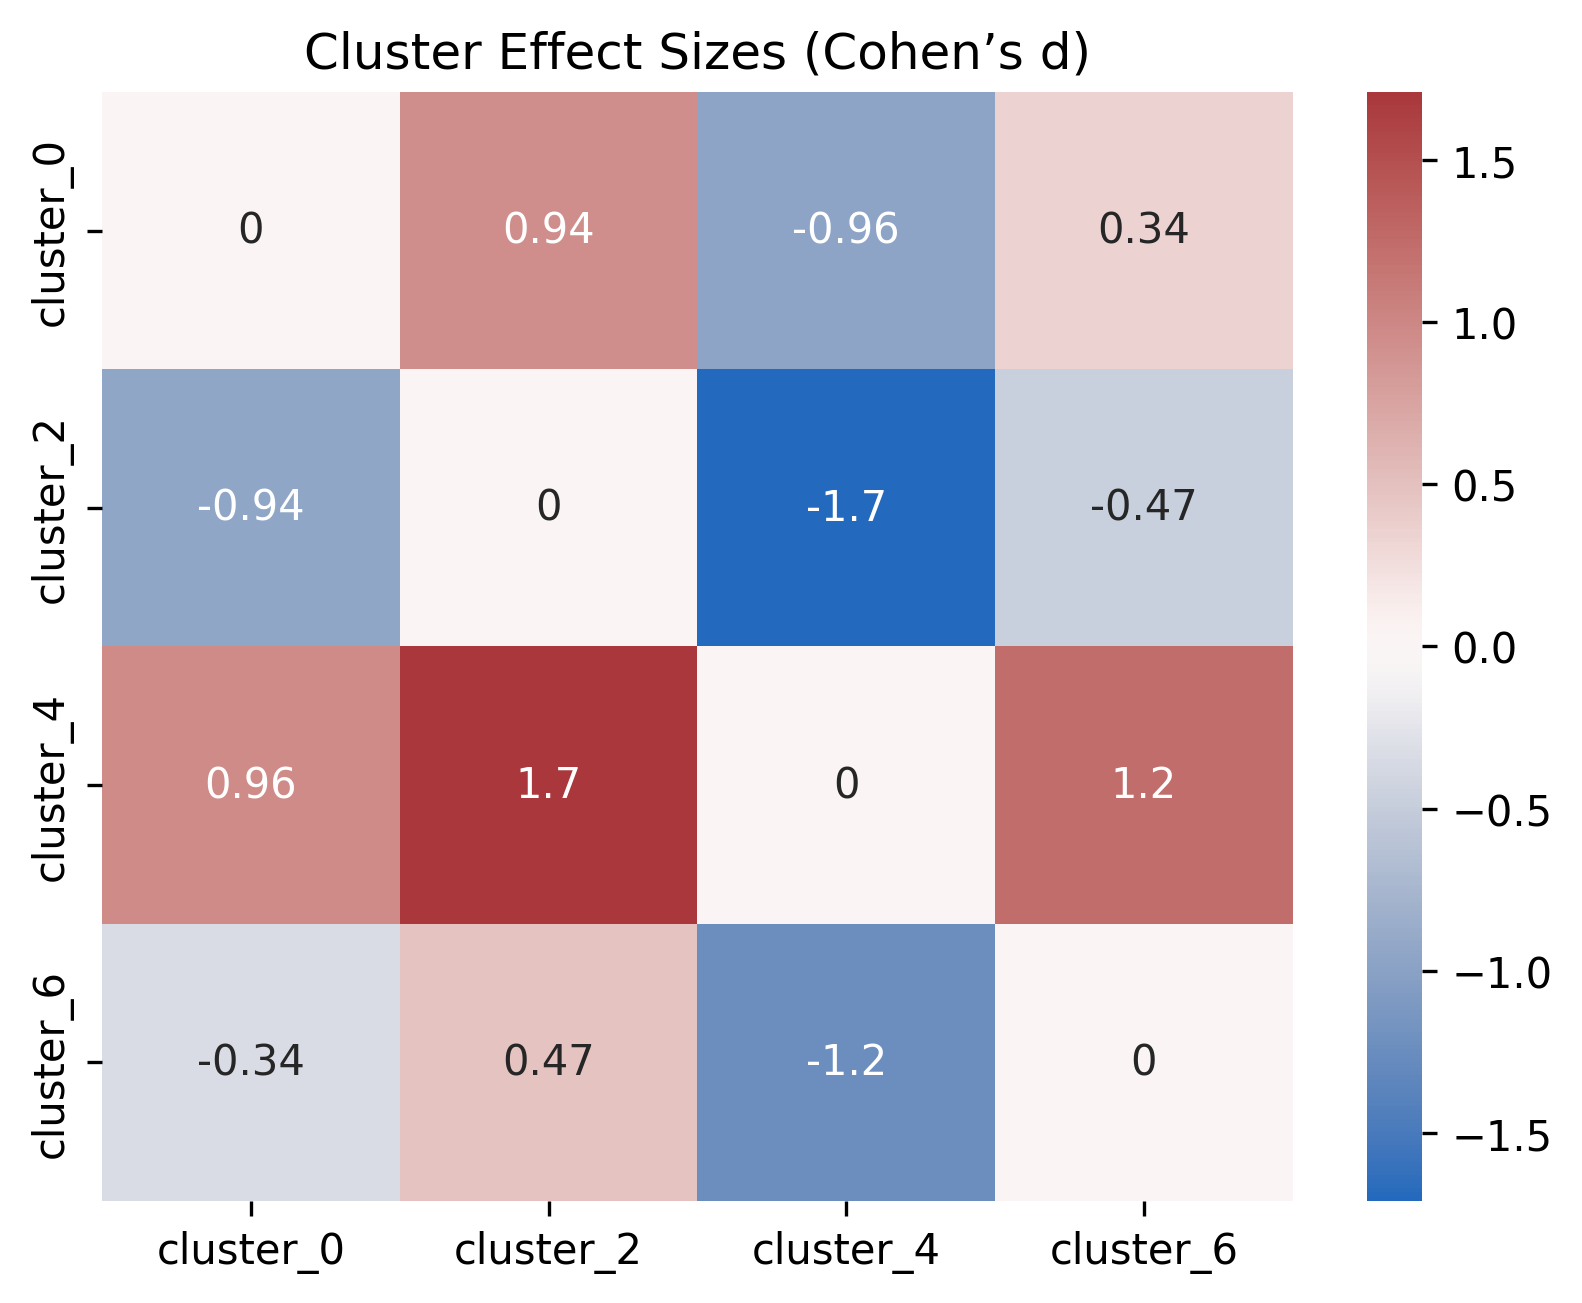
\includegraphics[width=0.8\textwidth]{effect-sizes.png}
    \caption{Effect-size estimates across clusters displaying Cohen's $d$ variation profiles.}
    \label{fig:effects-sizes}
\end{figure}

\begin{figure}[htbp]
    \centering
    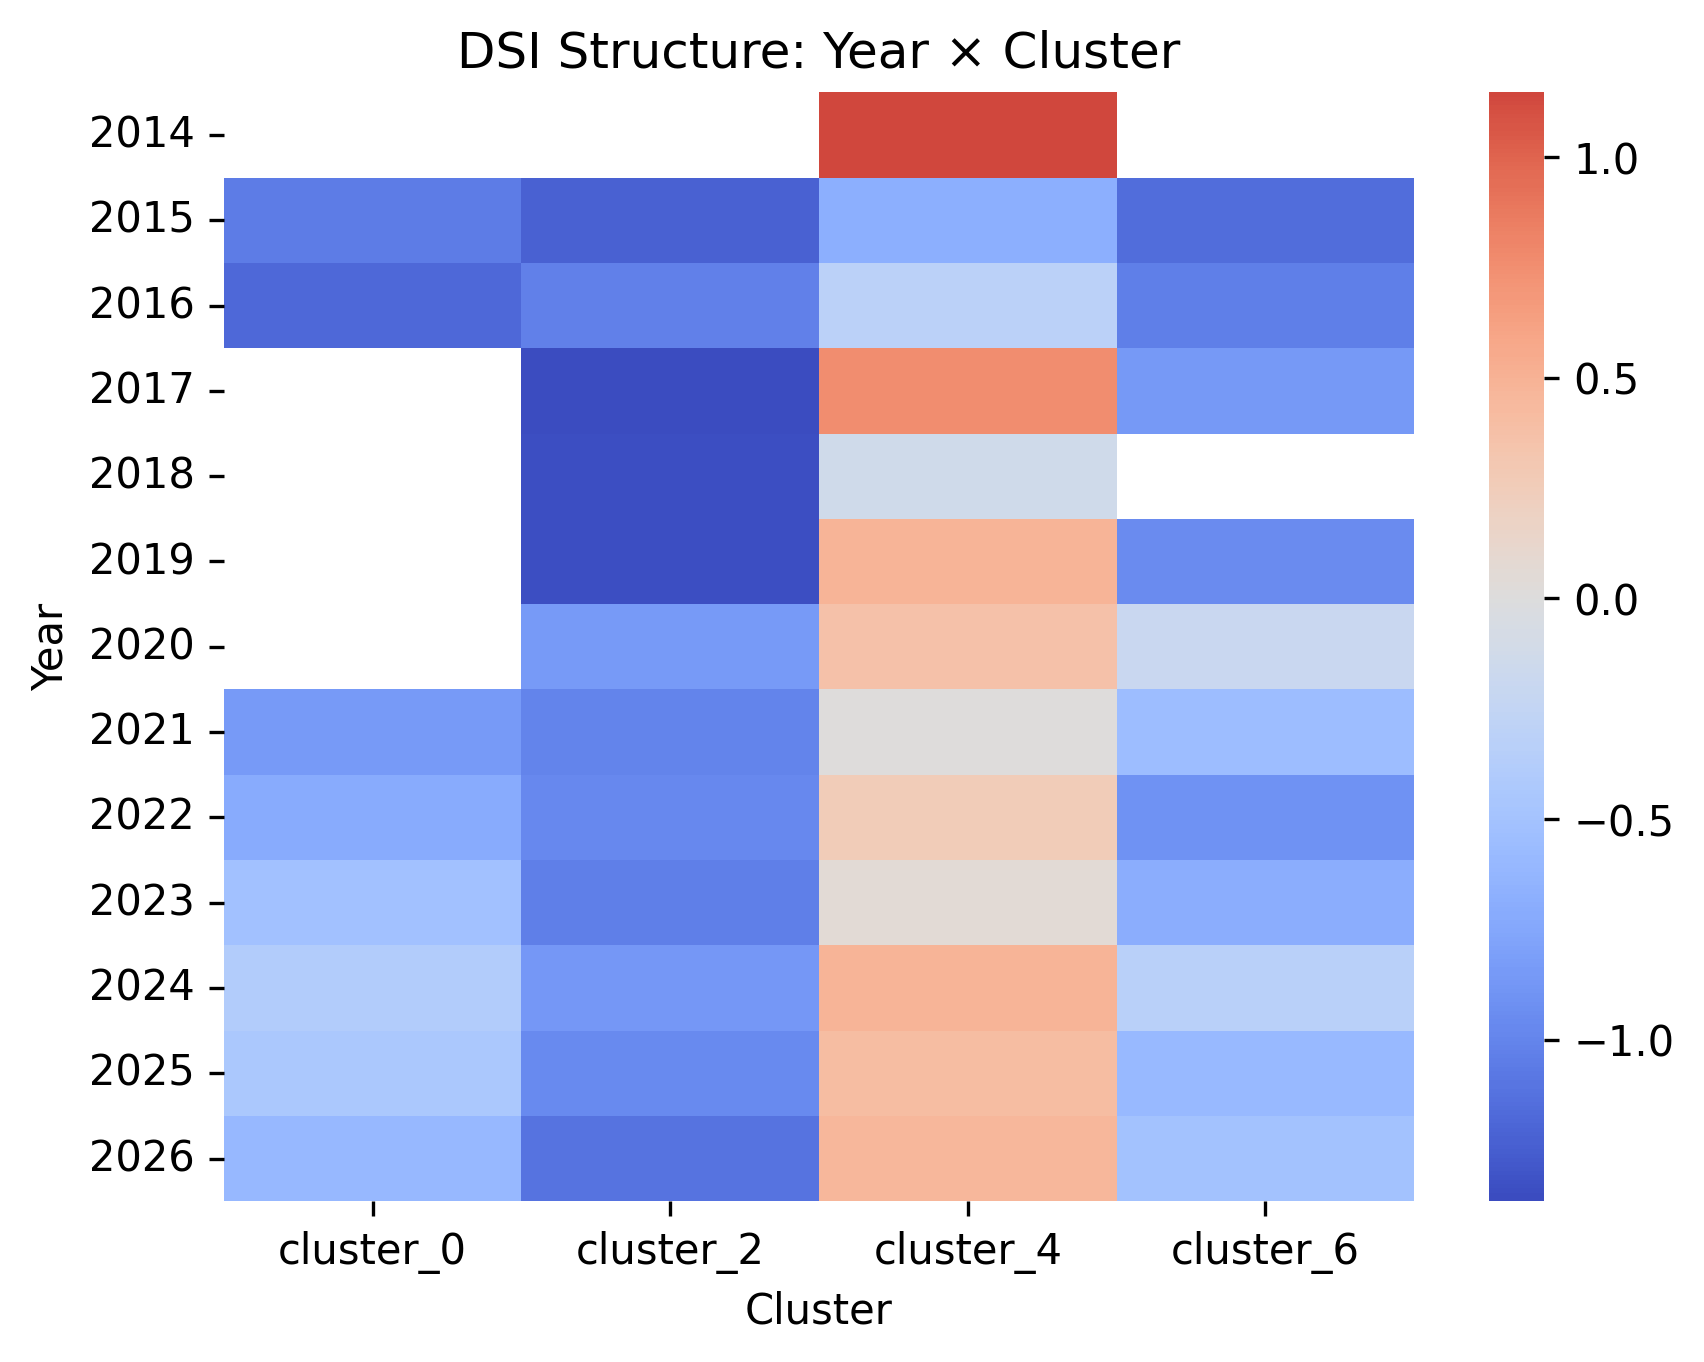
\includegraphics[width=0.8\textwidth]{heatmap.png}
    \caption{Structural density matrix tracking cluster-to-channel communication trajectories from 2014 to 2026.}
    \label{fig:heatmap}
\end{figure}

\subsection{Mixed-Effects Model}
As detailed in table~\ref{tab:model_comparison_metrics}, mixed-effects models outperform the aggregate OLS specification, indicating strong channel-level variance. 

\begin{table}[htbp]
\centering
\caption{Model comparison metrics between OLS baseline and mixed-effects specifications.}
\label{tab:model_comparison_metrics}
\begin{tabular}{lcc}
\toprule
\textbf{Model} & \textbf{AIC} & \textbf{BIC} \\
\midrule
OLS Full      & 672.48 & 706.34 \\
Mixed Effects & 653.45 & 695.78 \\
\bottomrule
\end{tabular}
\end{table}

The predicted trajectories from the mixed-effects model are presented in figure~\ref{fig:mixed-effects}. This figure illustrates the relative evolution of the model terms and further demonstrates the descriptive superiority of the mixed-effects specification over the corresponding OLS baseline model. The lower AIC (653.45) and BIC (695.78) values in the mixed-effects model compared to the OLS baseline signify a statistically superior fit, justifying the need for channel-level analysis. These metrics indicate that a single trend line is inadequate and that the data requires a multi-level approach due to divergent communication trajectories across different media channels.
	
\begin{figure}[htbp]
    \centering
    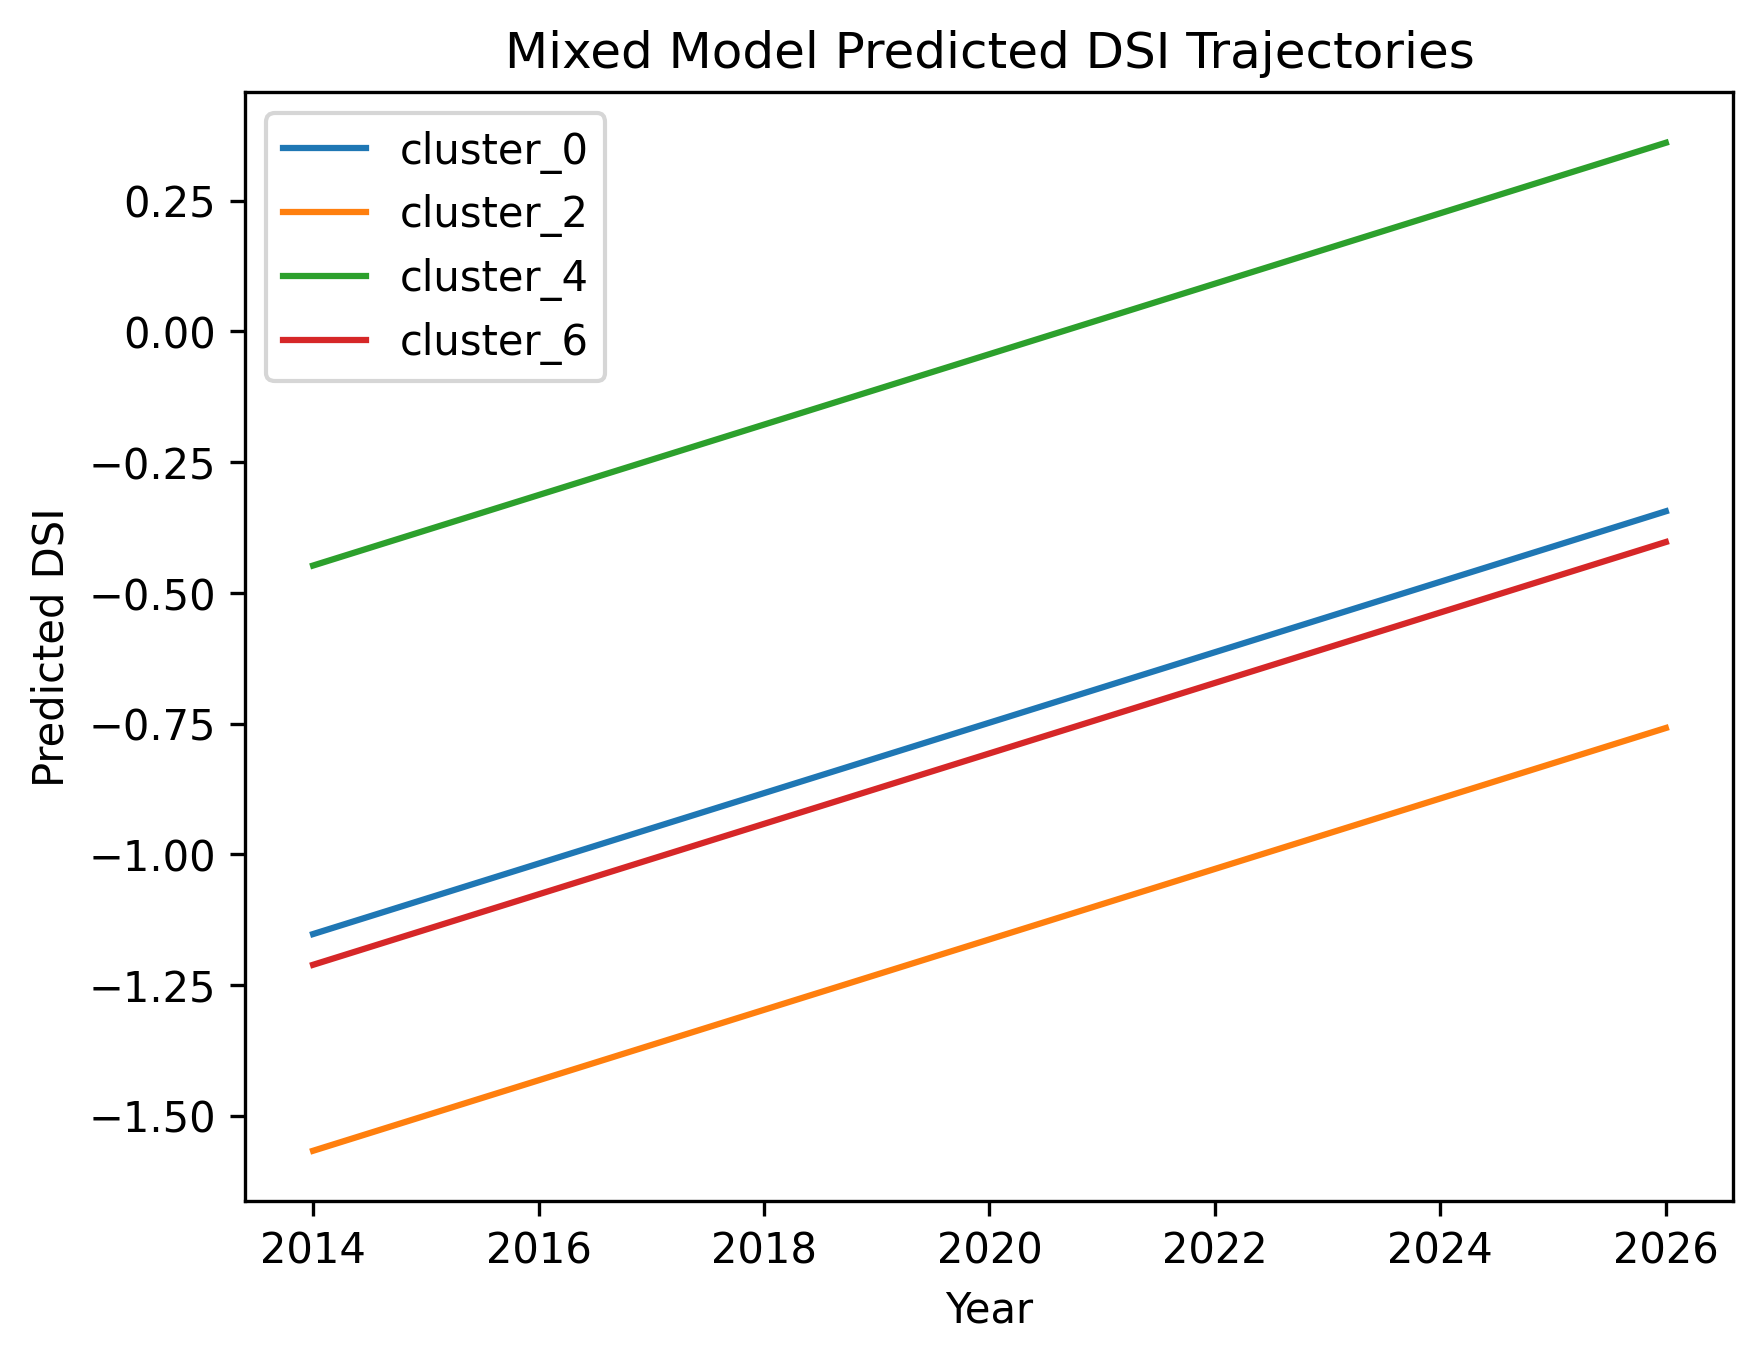
\includegraphics[width=0.8\textwidth]{mixed-effects.png}
    \caption{Mixed-effects model predicted DSI trajectories across independent cluster classifications.}
    \label{fig:mixed-effects}
\end{figure}

This progressive macro-level paradigm shift and structural alignment across institutional categories is empirically map-indexed across the broader bibliometric field in figure~\ref{fig:yoga_trends_2014_2026}. It is clear the trend toward yogic informed sustainable governance has increased over time. While the increase in neuro-immunomodulation from 2019 onwards has also outpaced the more stable pulmonary therapeutic focus.


\section{Discussion}

\subsection{Structural Differentiation and Institutional Partitioning (H1)}
The statistical verification of hypothesis \textbf{H1} ($F = 142.62, p < 0.001$) demonstrates that the identified discourse clusters are not arbitrary semantic groupings. Rather, they represent structurally independent communicative regimes deeply embedded within specific channel infrastructures. The stark variation in DSI visualised in the boxplot distribution of figure~\ref{fig:dsi_distribution_boxplots} tracks a highly partitioned symbolic arena. 

\begin{figure*}[htbp]
\centering
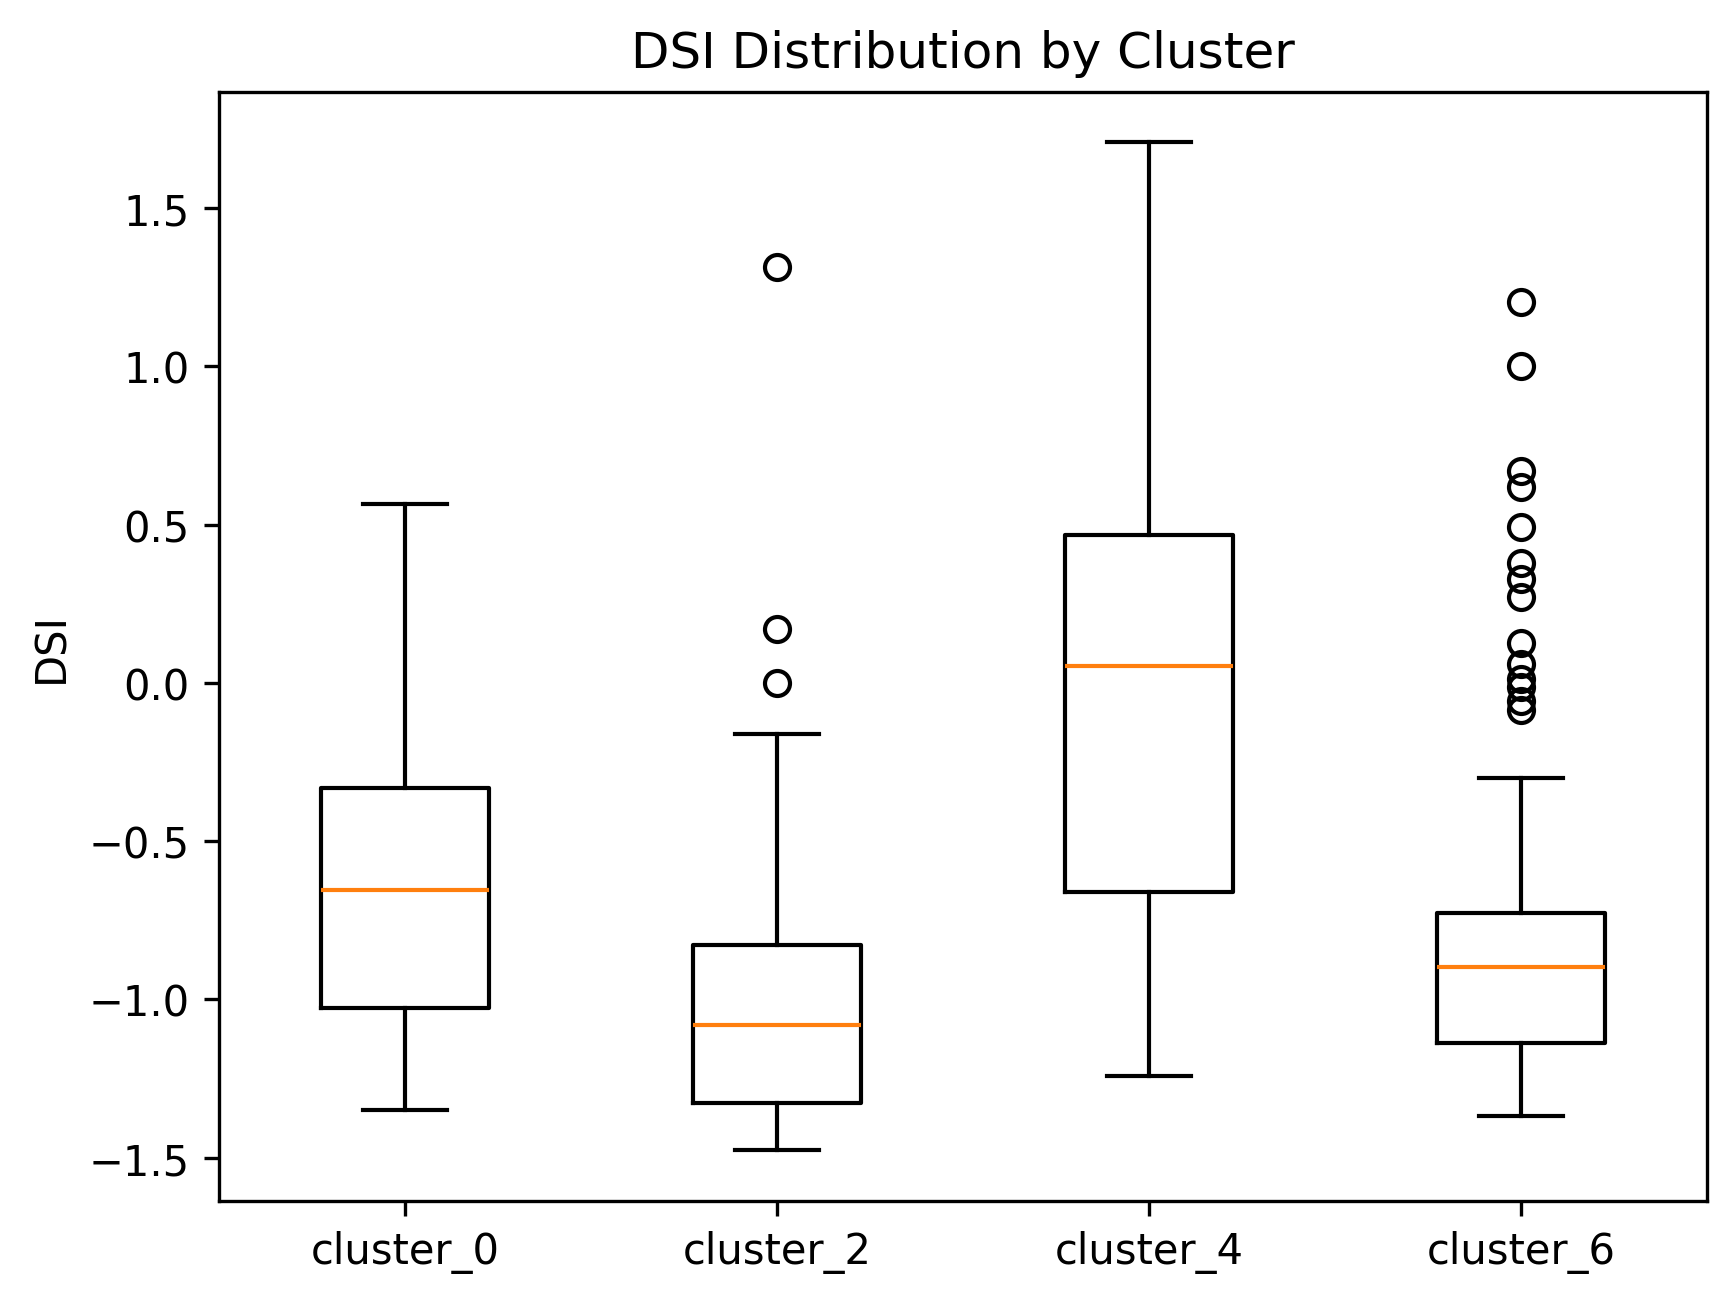
\includegraphics[width=0.85\textwidth]{dsi_distribution_boxplots.png}
\caption{Distribution of the DSI across the four identified discourse clusters, highlighting distinct rhetorical profiles across institutional contexts.}
\label{fig:dsi_distribution_boxplots}
\end{figure*}

This systematic variation is heavily driven by source channel type ($\chi^2(27) = 91.98, p < 0.001$), confirming a strict institutional division of labor across the IDY ecosystem. State policy organs and diplomatic channels (dominant in \textit{Cluster 4}) leverage a highly complex, formalised semantic structure. Conversely, mass media platforms (\textit{Cluster 0}) and civil-society wellness hubs (\textit{Cluster 2}) deploy less complex, descriptive linguistic structures to satisfy localized or commercial logics. This empirical divergence supports the theoretical contentions of Merkel and McCartney, showing that the shared global calendar event does not generate a monolithic narrative, but functions instead as a multi-centric arena where diverse actors utilize a flexible vocabulary to pursue distinct, decoupled institutional objectives.

\subsection{Temporal Reconfiguration and Governance Alignment (H2)}
The overall upward trajectory of the DSI across the twelve-year timeline ($\rho = 0.248, p < 0.001$) provides robust backing for \textbf{H2}, capturing a macro-level formalisation of the IDY discursive field. This structural transformation tracks a clear transition from early, foundational wellness claims to complex, international governance architectures. 

This longitudinal evolution is structurally mapped out in {table~\ref{tab:idy_themes}}, which charts the historical transition from pre-2014 localized fitness themes toward macro-environmental policies between 2019 and 2026. As visualized in the keyword frequency mapping of \text{figure 1}, the narrative uses highly accessible, organic baselines (\textit{nature}, $n=227$; \textit{lifestyle}, $n=220$) as a rhetorical bridge to systematically integrate formal policy frameworks (\textit{sdg}, $n=36$; \textit{climate}, $n=24$). This structural alignment converts individual, spiritual self-care constraints directly into state-sponsored systemic directives. This structural transition is macro-empirically validated by recent interdisciplinary health governance models. In their structural equation modeling of global mind-body practices, \citet{zhou2026yoga} establish that a practice's documented clinical health benefits exert a powerful, direct positive effect on its subsequent public policy integration ($\beta = 0.63, p < 0.001$). By capitalizing on this underlying evidence-to-policy translation mechanism, the Modi administration effectively converts yoga's immense global biomedical validity pool into an unassailable rhetorical launchpad for international environmental mandates.

 This empirical trend provides a clear linguistic blueprint of the Indian state's ``guru governmentality''. By standardizing and scaling up civilizational tropes like \textit{aparigraha} to align directly with UN targets like SDG 12 and 13 (\text{table 1}), the administration of Prime Minister Modi constructs a highly sophisticated, mediatized apologia designed to position India as the moral, cosmic steward (\textit{vi\'{s}va-guru}) of international environmental frameworks like Mission LiFE.

The geopolitical origins of this bibliometric dataset expose the top-down nature of this network. Within the non-clinical literature, India holds an absolute monopoly, driving 138 Governance papers and 37 Sustainability papers, compared to the United States (28 and 10 respectively). In a database historically dominated by Western and Chinese institutional funding, this stark inversion proves that yoga's evolution into an environmental narrative is a state-financed intellectual project. By leveraging the Ministry of AYUSH and funding traditional systems like Unani and Siddha, the Modi administration uses peer-reviewed science as a transponder to project its civilizational statecraft globally.

\subsection{Segmented Trajectories and Discursive Fragmentation (H3)}
Crucially, the interaction and mixed-effects models backing \textbf{H3} demonstrate that this institutionalization process is profoundly uneven across the corpus. As illustrated by the predicted trajectories in \text{figure 4} and the temporal heat matrix in \text{figure 5}, the structural complexity of IDY communication does not advance uniformly. 

The system instead undergoes a process of institutional partitioning, characterized by divergent longitudinal paths. State policy channels and international diplomatic entities (\textit{Cluster 4} and \textit{Cluster 6}) show powerful, statistically significant positive trends over time, continuously intensifying the structural integration of macro-governance language. In stark contrast, commercial wellness circles and grassroots yoga organizations (\textit{Cluster 2}) remain statistically flat and static across the 2014--2026 window. Rather than engaging with evolving policy targets, these actors reiterate basic, metaphor-driven slogans in a formulaic manner.

This persistent divergence highlights the structural contours of the ``culture-policy paradox'' identified in modern cross-cultural communication frameworks \cite{zhou2026yoga}. Quantitative modeling reveals that highly decentralized, market-driven cultural dissemination modes carry a significant negative path coefficient regarding formal institutional policy integration ($\beta = -0.30, p = 0.014$), primarily because modern bureaucratic frameworks demand highly standardized, predictable, and controllable intervention protocols. The state-aligned channels in Cluster~4 and Cluster~6 are explicitly engineered to bypass this structural friction. By wrapping the fluid, adaptive traditions of practice inside a rigid, highly formalized macro-governance vocabulary, state organs insulate the signal from the domestic market's cultural dilution, guaranteeing its frictionless assimilation into international institutional frameworks.

 The mixed-effects model comparison (\text{Table 5}) confirms that these patterns are not driven by a handful of loud or prolific content channels, but reflect deep, persistent sub-community divisions across the field. This uneven development proves that while the Indian state attempts to amplify its soft-power signal globally, that signal is continuously diffracted, segmented, and insulated by the independent internal communicative logics of civil society.


\subsection{Synthesis}

Taken together, the results indicate that IDY discourse operates as a dynamically structured system shaped by both institutional differentiation and temporal evolution. Rather than a unified global discourse, the corpus reveals a layered configuration of semi-autonomous discourse regimes that evolve along distinct trajectories while remaining loosely coupled within a shared symbolic event.

\subsection{The Disembodied Grid: From Ambient Gaze to Ambient Guruship}
This structural formalization and top-down policy integration require a critical re-evaluation of how religious charisma and political authority scale across modern digital media landscapes. Rather than operating via traditional, localized, or embodied lineage transmission (\textit{parampar\={a}}), the IDY ecosystem operates as a highly sophisticated, distributed grid of state power.

This mechanism is best understood by tracking the conceptual evolution from the macro-level \textit{ambient gaze} theorized by McCartney and Louren\c{c}o~\cite{mccartney2023} to the broader algorithmic framework of the \textit{ambient guru} advanced by Copeman's \textit{GuruAI: The Global Anthropology of the Transformation of Guruship in the Age of Artificial Intelligence} project~\cite{copeman2023,idega2026}. McCartney and Louren\c{c}o originally demonstrated that non-human material objects and digital media arrays can function as ubiquitous, interlinked nodes that broadcast a guru's continuous spatial attention -- behaving less like a localized person and more like an omnipresent ``Wi-Fi signal'' that conditions practitioner behaviors and signals unbridled social distinction.

When mapped onto our longitudinal dataset, this ambient architecture undergoes a profound technological and political upgrade, scaling into a mature manifestation of Copeman’s ``ambient guru'' ~\cite{copeman2012,idega2026}. Here, the traditional boundaries of religious authority are completely unmoored from physical proximity or biological containment. The IDY framework functions as a vast digital panopticon where individual state-aligned channels (such as the hyper-complex vectors in Cluster 4 and Cluster 6) act as localized digital transponders for a singular, disembodied ideological signal. 

Concurrently, the 7,978 papers mined from the NIH PubMed index serve as the literal epistemological infrastructure of this disembodied grid. When our text-contrast matrix strips away the clinical background noise, the phrases that rise to the top -- ``School-Based,'' ``Medical Education,'' ``Environmental Factors,'' and ``Climate Change' -- expose exactly how the ambient guru operates. The grid embeds state directives directly into international health, educational, and environmental curricula. The individual practicing a school-based breathing protocol for ``emotion regulation'' is no longer just engaging in localized self-care. 

As empirically verified by the dual-axis growth curves in figure~\ref{fig:niche_growth_trajectory} and the absolute domination of Indian institutional hub data in table~\ref{tab:model_comparison_metrics}, they are behaving as an active node inside a distributed panopticon of state power. The material mechanics of this panopticon are anchored to profound economic asymmetries in global practice delivery. While community-based public provision models, such as those governing state-led Tai Chi frameworks, prioritize equity through a high proportion of free or fully subsidized programs ($65.1\%$), the globalized market layout of yoga skews heavily toward commercialized, consumer-funded spaces characterized by significantly higher localized session costs ($25.6 \pm 12.3$ USD/hour) \cite{zhou2026yoga}. The ambient grid exploits this exact commercial capillarity; by inserting state-prescribed definitions of eco-citizenship directly into a premium global wellness economy, the state transforms a costly, localized lifestyle commodity into a ubiquitous vector of geopolitical alignment.

 This architecture allows the Indian state to project Modi’s political and civilizational guruship (\textit{vi\'{s}va-guru}) globally without requiring his active, embodied presence in every localized arena, transforming a centralized state-branding initiative into an ambient, everyday social environment automated by code, media interfaces, and institutionalized narrative structures. Though, perhaps nothing could be the sci-fi like mediatization of Modi than being holographically projected into villages strewn across the \textit{darkness} during the 2014 election cycle \cite{deshgujarat2013modi,deb2024twilight}.


\subsection{Discursive Institutionalization}

The findings suggest that IDY has undergone a process of discursive institutionalization during the period under investigation. Across the corpus, discourse becomes increasingly differentiated, organized, and structured over time. This pattern is reflected in both the clustering results and the temporal analyses, which indicate that distinct communicative forms emerge and stabilize as IDY develops from a newly established international event into a recurring global event.

Institutionalization refers not merely to the growth of participation but to the emergence of relatively stable communicative practices, expectations, and organizational forms. In the early years of the corpus, discourse surrounding IDY exhibits comparatively low levels of differentiation and frequently emphasizes foundational themes such as awareness, participation, legitimacy, and public promotion. Over time, however, discourse communities become increasingly specialized. Different actors begin to emphasize distinct objectives, including public health, education, diplomacy, cultural heritage, community engagement, and governmental policy. This diversification suggests that IDY has evolved from a singular commemorative initiative into a broader institutional field containing multiple communicative centres.

These findings are consistent with theories of institutionalization, which predict increasing differentiation and specialization as social initiatives mature and become embedded within organizational structures. Rather than remaining a one-time symbolic event, IDY appears to have generated a durable communicative infrastructure that reproduces itself annually through media coverage, public events, governmental initiatives, and institutional participation.


\subsection{Emergence of a Discursive Field}

The clustering analysis demonstrates that IDY is best understood not as a unified discourse but as a heterogeneous discursive field, which is composed of various public and private actors operating according to different communicative logics. Although all corpus documents are connected through reference to IDY, they nevertheless exhibit substantial variation in linguistic structure, thematic emphasis, and discursive orientation.

This finding challenges representations of IDY as a singular global movement or coherent ideological project. Instead, the corpus suggests the coexistence of multiple overlapping discourse communities. It appears to start with government agencies employing IDY to communicate policy objectives and national initiatives. Downstream from this are educational institutions emphasizing awareness and learning such as yoga oriented institutions and primary schools, which share videos of students performing the CYP. Adjacent to this are the various health-oriented actors who focus on wellness outcomes and therapeutic benefits through promoting their own brand of yoga. These signals are amplified through many media organizations which frame IDY as a newsworthy event, while cultural organizations position it within broader narratives of heritage, identity, and social participation.

From this perspective, IDY functions as a discursive arena. From within this arena, diverse actors negotiate for legitimacy to calibrate meaning and identity. This is more of a competitive space, rather than a single stage from which a single unified message is transmitted from a central source. The resulting communicative ecology is therefore characterized by plurality, contestation, and differentiation. This interpretation aligns with broader approaches in discourse studies that view public events as sites of meaning-making rather than as vehicles for the transmission of fixed ideological content. Yet, even though the Indian state attempts to amplify its soft power, cultural diplomacy ambitions to influence global governance the state-driven signal is diffracted through the multiplicity of actors anchored to IDY. The identification of distinct discourse communities is particularly important because it demonstrates that IDY has become capable of accommodating multiple institutional agendas simultaneously. Such flexibility may help explain its continued expansion and durability across different national and organizational contexts.


\subsection{Uneven Temporal Development}

A second important finding concerns the uneven temporal development of discourse communities. The longitudinal analyses reveal that institutionalization is not occurring uniformly across the corpus. Some clusters display strong positive temporal trajectories, while others remain relatively stable or exhibit more limited rates of change. This result suggests that different sectors of the IDY communicative field are evolving according to distinct developmental logics. While certain discourse communities appear to be rapidly expanding and becoming more structurally differentiated, others have reached a comparatively stable configuration, where metaphor-driven slogans, for example, are repeated in a mantra-like fashion. However, the significant interaction effects observed in both regression and mixed-effects models indicate that temporal change is conditioned by cluster membership rather than operating as a uniform process affecting all discourse equally.

The existence of uneven developmental trajectories has important theoretical implications. It suggests that institutionalization should not be conceptualized as a singular linear process. Rather, IDY appears to consist of multiple partially autonomous discourse communities, each responding differently to changing political, social, cultural, and media conditions. This finding is consistent with contemporary theories of institutional fields, which emphasize heterogeneity, competition, and differentiated rates of organizational change. Moreover, the results imply that future analyses of IDY should move beyond aggregate measures of growth or participation and instead examine the specific trajectories of individual discourse communities. Such an approach may provide a more nuanced understanding of how cultural initiatives evolve through time.


\subsection{Beyond Advocacy Scholarship}

The present study also contributes to the emerging literature on IDY itself. Existing scholarship has tended to focus on three primary themes: health promotion, cultural diplomacy, and political interpretation. Much of this work is either explicitly promotional, documenting the benefits of yoga and public participation, or descriptive, reporting events and institutional activities associated with IDY. A smaller body of scholarship has investigated IDY's role in promoting ethno-nationalism through magnifying the soft power instrumentalization of its political symbolism. Still, relatively little research has treated IDY as an empirical object of discourse analysis. Instead, the predominant emphasis has been on evaluating the initiative's health outcomes, diplomatic significance, or ideological implications rather than investigating the communicative structures through which those meanings are produced and circulated.

This is partly why the present study has adopted the approach of avoiding asking whether IDY is beneficial, effective, or politically desirable. Instead, it examines how discourse surrounding IDY is organized and how that organization changes over time. Thus, by combining corpus construction, unsupervised clustering, longitudinal analysis, and statistical modelling, this present study has purposely shifted attention away from normative evaluation to empirical investigation. It is important to make this distinction because it allows IDY to be analyzed as a communicative ecosystem in its own right. Thus, from this perspective, questions concerning health promotion, nationalism, cultural diplomacy, or public participation become observable components of a broader discursive field rather than predetermined explanatory frameworks. Adopting such an approach opens up new possibilities for the study of, not only IDY but, contemporary cultural initiatives, public rituals, and globally mediated commemorative events. At broader levels, the findings demonstrate the value of computational approaches for investigating large-scale cultural phenomena. By analysing discourse longitudinally and at scale, researchers can move beyond isolated case studies, anecdote and opinion to examine the processes through which institutional narratives emerge, stabilize, and transform over time. In this respect, IDY provides a useful case study of how cultural, political, and health-related discourses become institutionalized within contemporary digital media environments.


\section{Limitations}

Several limitations should be acknowledged when interpreting the findings of this study.

First, due to the extraction limitations, the corpus exhibits uneven temporal coverage across the study period. Despite the final dataset spanning 2014--2026, the number of harvested transcripts varies considerably between years. This is perhaps somewhat due to the earlier years of the corpus containing relatively fewer documents, while later years are represented by substantially larger samples. This imbalance reflects both the historical development of IDY itself and the availability of digital media content. Consequently, yearly comparisons should be interpreted cautiously, particularly for years with limited observations.

Second, the corpus is platform-dependent. The dataset was constructed primarily from YouTube transcripts, creating a specific digitally mediated environment. While YouTube provides broad coverage of IDY-related activities, it does not capture the entirety of the communicative field. Important forms of discourse circulating through television broadcasts, print media, governmental documents, other social media platforms, organizational reports, and offline events remain outside the scope of the present analysis. Even though they have, to various degrees, been consulted. The corpus should therefore be understood as a substantial but necessarily partial representation of IDY discourse. For example, a great deal of data has been harvested from both Twitter and Instagram. However, the decision was made to focus this paper on YouTube.

Third, the dataset exhibits a degree of linguistic bias. Although efforts were made to include multilingual material where available, the final corpus is disproportionately composed of English-language transcripts due to the greater availability and accessibility of English subtitles and transcripts on the platform. One of the biggest issues related to the scraping of transcripts was choosing which languages to include. The issue of collecting all available languages meant collecting machine translated versions, or triggering 429 issues through sending too many requests. As a result, the findings may underrepresent communicative practices occurring in Hindi and other regional languages, as well as forms of discourse intended primarily for local rather than international audiences.

Fourth, the DSI developed in this study is designed to capture structural variation within discourse rather than semantic meaning in a narrow sense. This is why there is virtually no discourse presented in this paper. Following the semantic waves is a different topic for a future paper. Instead, the index identifies patterns of differentiation, organization, and positioning among discourse communities, avoiding directly measuring ideological content, sentiment, persuasion, or political orientation. Consequently, the DSI values should be interpreted as indicators of discursive structure rather than as direct measures of substantive meaning.

Fifth, the study relies upon automated transcript extraction and computational text-processing procedures. Although extensive cleaning, validation, and quality-control measures were implemented throughout corpus construction, transcript-based research inevitably contains levels of noise. These arise from subtitle errors, transcription inaccuracies, metadata inconsistencies, and platform-specific artefacts. Even though significant attention was paid to limiting these factors, it is hoped that they will be unlikely to alter the overall patterns identified in the analysis. Still, there  may be an influence upon individual documents and local cluster assignments.

Finally, the clustering procedures employed in this study are just one way to represent possible interpretation of the latent structure of the corpus. There are other ways to potentially approach this analytical frame and topic through adopting alternative embedding models, clustering algorithms, preprocessing strategies, or parameter selections. Obviously, different approaches may produce somewhat different cluster boundaries, which would alter the results. Nonetheless, the objective of the analysis has not been to identify a single definitive classification of IDY discourse. Instead, it has attempted to reveal robust patterns of differentiation and temporal development within a large and heterogeneous corpus.

Despite these limitations, the consistency of the observed temporal trends across multiple statistical procedures, including analysis of variance, regression modelling, and mixed-effects models, suggests that the principal findings are unlikely to be artefacts of a particular methodological choice. Therefore, it would be interesting to reframe this same corpus with modulated analytical metrics to see what results might emerge.

\section{Conclusion}
This study presents a longitudinal computational critique of the International Day of Yoga (IDY) corpus from its inception through 2026, mapping its structural transition from a global wellness event into a highly complex, multi-tiered discursive field. Utilizing an integrated mixed-methods framework spanning 509 localized media transcripts and 1,758 policy artifacts cross-validated by 7,978 peer-reviewed NIH PubMed records, these empirical results challenge the prevailing baseline of normative, uncritical advocacy scholarship \cite{kamal2024yoga,sadineni2024reimagining}. Rather than broadcasting a singular, coherent message of cosmic or physical harmony, the IDY communicative ecosystem is structurally defined by sharp institutional partitioning ($F = 142.62, p < 0.001$), persistent sub-community divisions, and highly uneven temporal trajectories ($\rho = 0.248, p < 0.001$). 

This longitudinal modeling confirms a dual-action mechanism underlying the modern manifestation of ``guru governmentality.'' On the front lines of digital media public diplomacy, the Indian state uses platforms like YouTube to project an accessible, personalized framing of nature and lifestyle shifts. Simultaneously, behind the scenes of scientific infrastructure, the state has systematically retooled civilizational tropes to colonize global peer-reviewed biomedical and ecological literature. By engineering an explicit rhetorical bridge between classical terminology and international development metrics, state organs actively overcome the traditional ``culture-policy paradox'' ($\beta = -0.30$) that otherwise limits fluid, market-driven cultural traditions from achieving formal policy integration \cite{zhou2026yoga}. This top-down diplomatic signal undergoes significant diffraction when filtered through global channels, showing that discursive institutionalization does not inherently result in ideological homogenization. Instead, the IDY field proceeds through structured fragmentation, allowing state-aligned policy channels to aggressively build complex governance narratives over time, while grassroots networks remain statically anchored to basic wellness tenets.

Ultimately, the long-term viability and diplomatic durability of the IDY rest precisely upon this plastic structural flexibility -- its unique capacity to accommodate competing agendas simultaneously without collapsing under a forced uniformity. By deploying an ambient guru framework, the Indian civilizational state successfully exploits globalized, neoliberal wellness markets \cite{sen2026yoga}, transforming a centralized state-branding initiative into an omnipresent, automated everyday social environment. Methodologically, this investigation illustrates the robust utility of computational sociology to move beyond descriptive word-frequency counts. By testing explicit inferential hypotheses longitudinally and at scale, this study provides a template to directly model the processual dynamics through which state-driven cultural initiatives, public rituals, and globally mediated commemorative events become stabilized, diffracted, and automated within modern digital media environments.


\clearpage





\newpage





\textbf{\large Declaration}

No funding was received to assist with the preparation of this manuscript.
The authors have no relevant financial or non-financial interests to disclose.

\textbf{\large Data Availability Statement}

The datasets generated by the survey research during and/or analyzed during the current study are available in the GitHub repository, \url{https://github.com/psdmcc/idy-corpus-analysis/tree/main}.

\textbf{Use of AI}

ChatGPT and Google AI were used to workshop the analytical design and flow, debug python scripts, build the Bibtex file, and with understanding the results of the analysis.


\bibliographystyle{unsrtnat}
\begin{thebibliography}{65}
\providecommand{\natexlab}[1]{#1}
\providecommand{\url}[1]{\texttt{#1}}
\expandafter\ifx\csname urlstyle\endcsname\relax
  \providecommand{\doi}[1]{doi: #1}\else
  \providecommand{\doi}{doi: \begingroup \urlstyle{rm}\Url}\fi

\bibitem[Copeman and Ikegame(2012)]{copeman2012}
Jacob Copeman and Aya Ikegame.
\newblock Guru logics.
\newblock \emph{HAU: Journal of Ethnographic Theory}, 2\penalty0 (1):\penalty0
  289--336, 2012.
\newblock \doi{10.14318/hau2.1.014}.

\bibitem[Merkel(2015)]{merkel2015}
Udo Merkel.
\newblock Making sense of identity discourses in international events,
  festivals and spectacles.
\newblock In Udo Merkel, editor, \emph{Identity Discourses and Communities in
  International Events, Festivals and Spectacles}, Leisure Studies in a Global
  Era, pages 3--33. Palgrave Macmillan, London, 2015.

\bibitem[Mokdad(2025)]{mokdad2025}
Mohamad Mokdad.
\newblock The rise of soft power in modern diplomacy.
\newblock In Mohamad Zreik, editor, \emph{Innovations and Tactics for 21st
  Century Diplomacy}, pages 29--50. IGI Global, New York, 2025.
\newblock \doi{10.4018/979-8-3693-6074-3.ch002}.

\bibitem[Chandra(2026)]{chandra2026}
Ramesh Chandra.
\newblock India’s cultural diplomacy in the modi era: Soft power as a
  strategic tool in global governance.
\newblock \emph{ShodhSamajik}, 3\penalty0 (1):\penalty0 170--177, 2026.
\newblock \doi{10.29121/ShodhSamajik.v3.i1.2026.95}.

\bibitem[Otto(2025)]{otto2025}
L.~Otto.
\newblock India’s use of yoga in diplomacy.
\newblock \emph{The Review of Faith \& International Affairs}, 23\penalty0
  (2):\penalty0 1--13, 2025.
\newblock \doi{10.1080/15570274.2025.2491265}.

\bibitem[Bhagwat(2019)]{bhagwat2019}
Shonil Bhagwat.
\newblock Can yoga help us achieve sustainable development goals?
\newblock Open University, 2019.
\newblock Retrieved June 28, 2026, from
  \url{https://www.open.edu/openlearn/health-sports-psychology/health/can-yoga-help-us-achieve-sustainable-development-goals}.

\bibitem[Hjarvard(2008)]{hjarvard2008}
Stig Hjarvard.
\newblock The mediatization of society: A theory of the media as agents of
  social and cultural change.
\newblock \emph{Nordicom Review}, 29\penalty0 (2):\penalty0 105--134, 2008.
\newblock \doi{10.1515/nor-2017-0181}.

\bibitem[Jagannathan et~al.(2026)Jagannathan, More, Kumar, Nishitha, Nagendra,
  Gangadhar, and Rao]{jagannathan2026}
Aarti Jagannathan, Pooja More, Vinod Kumar, J.~Lakshmi Nishitha, H.~R.
  Nagendra, B.~N. Gangadhar, and Raghavendra Rao.
\newblock Yoga as an eco-therapy for achieving united nations sustainable
  development goals: An explorative study.
\newblock \emph{International Journal of Yoga}, 19\penalty0 (1):\penalty0
  45--52, 2026.
\newblock \doi{10.4103/ijoy.ijoy_72_25}.

\bibitem[Lejano et~al.(2013)Lejano, Ingram, and Ingram]{lejano2013}
Raul Lejano, Mrill Ingram, and Helen Ingram.
\newblock \emph{The Power of Narrative in Environmental Networks}.
\newblock MIT Press, Cambridge and London, 2013.

\bibitem[de~Neufville and Barton(1987)]{deneufville1987}
Judith de~Neufville and Stephen Barton.
\newblock Myths and the definition of policy problems: An exploration of home
  ownership and public-private partnerships.
\newblock \emph{Policy Sciences}, 20\penalty0 (3):\penalty0 181--206, 1987.

\bibitem[Bonikowski and Nelson(2022)]{bonikowski2022}
Bart Bonikowski and Laura~K. Nelson.
\newblock From ends to means: The promise of computational text analysis for
  theoretically driven sociological research.
\newblock \emph{Sociological Methods \& Research}, 51\penalty0 (4):\penalty0
  1937--1977, 2022.
\newblock \doi{10.1177/00491241221123088}.

\bibitem[Bhattacharyya et~al.(2015)Bhattacharyya, Patil, and
  Muninarayana]{bhattacharyya2015}
A.~Bhattacharyya, N.~J. Patil, and C.~Muninarayana.
\newblock Yoga for promotion of health: Conference held on international day of
  yoga 2015 at kolar.
\newblock \emph{Journal of Ayurveda and Integrative Medicine}, 6\penalty0
  (4):\penalty0 305--306, 2015.
\newblock \doi{10.4103/0975-9476.172425}.

\bibitem[Patil et~al.(2016)Patil, Venkatarathnamma, and
  RamchandraRao]{patil2016}
N.~J. Patil, P.~N. Venkatarathnamma, and S.~RamchandraRao.
\newblock Yoga for lifestyle diseases: Conference held on 2nd international day
  of yoga 2016 at kolar, india.
\newblock \emph{Journal of Ayurveda and Integrative Medicine}, 7\penalty0
  (4):\penalty0 261--262, 2016.
\newblock \doi{10.1016/j.jaim.2016.09.001}.

\bibitem[Manjunath(2023)]{manjunath2023}
N.~K. Manjunath.
\newblock The transformative impact of the international day of yoga.
\newblock \emph{International Journal of Yoga}, 16\penalty0 (1):\penalty0 1--4,
  2023.
\newblock \doi{10.4103/ijoy.ijoy_106_23}.

\bibitem[Mohan et~al.(2024)Mohan, Vadiraja, Moirangthem, et~al.]{mohan2024}
Raghavendra~Rao Mohan, Hosakote~Sanjeeva Vadiraja, Ghanapriyari Moirangthem,
  et~al.
\newblock Impact assessment of international day of yoga: Results from a
  cross-sectional survey.
\newblock \emph{Indian Journal of Yoga and Naturopathy}, 1\penalty0
  (1):\penalty0 24--29, 2024.
\newblock \doi{10.4103/ijyn.ijyn_6_24}.

\bibitem[Prasad et~al.(2025)Prasad, Mahesshwari, and Kaur]{prasad2025}
Urvashi Prasad, Ankeetaa Mahesshwari, and Mehek Kaur.
\newblock The research impact of international day of yoga: A scientometric
  analysis of yoga's global influence, 2025.
\newblock Retrieved June 20, 2026, from
  \url{https://naturopathyday.in/upload/Pahle%20India%20Yoga%20Book%20VI%2013-06-25.pdf}.

\bibitem[Zhou et~al.(2026)Zhou, Bojarczuk, Shen, Chen, Zhong, Chen, and
  Zhong]{zhou2026yoga}
H.~Zhou, A.~Bojarczuk, G.~Shen, S.~Chen, K.~Zhong, J.~Chen, and W.~Zhong.
\newblock Yoga and {Tai} chi: a cross-cultural comparative study of health
  benefits, cultural sustainability, and global public health implications.
\newblock \emph{Frontiers in Public Health}, 14:\penalty0 1746662, 2026.
\newblock \doi{10.3389/fpubh.2026.1746662}.

\bibitem[Sadineni and Shastri(2024)]{sadineni2024reimagining}
Nagarjuna Sadineni and Sandeep Shastri.
\newblock Reimagining {Sustainable Development Goals} and {IT} industry
  governance through ancient {Indian} concepts of "{Dharma} and {Yogakshema}".
\newblock \emph{Migration Letters}, 21\penalty0 (S2):\penalty0 1180--1190,
  2024.
\newblock ISSN 1741-8984.

\bibitem[Gautam and Droogan(2018)]{gautam2018}
Aakriti Gautam and Julian Droogan.
\newblock Yoga soft power: How flexible is the posture?
\newblock \emph{Journal of International Communication}, 24\penalty0
  (1):\penalty0 18--36, 2018.
\newblock \doi{10.1080/13216597.2017.1388829}.

\bibitem[Sen et~al.(2026)Sen, Mishra, Rajagopal, and Chakrabarti]{sen2026yoga}
Subhasis Sen, Mukunda Mishra, K.~Rajagopal, and Anjan Chakrabarti.
\newblock {Yoga}, neo-liberal society, and well-being industries: An
  exploration of global and indian perspectives.
\newblock In Subhasis Sen, Mukunda Mishra, K.~Rajagopal, and Anjan Chakrabarti,
  editors, \emph{Sports, Inclusion, and Peace: SDG-16 and India in
  Perspective}, pages 23--45. Springer Singapore, Singapore, 2026.
\newblock \doi{10.1007/978-981-92-1978-0_2}.

\bibitem[Miller(2020)]{miller2020}
Christopher~P. Miller.
\newblock Soft power and biopower: Narendra modi's "double discourse"
  concerning yoga for climate change and self-care.
\newblock \emph{Journal of Dharma Studies}, 3:\penalty0 93--106, 2020.
\newblock \doi{10.1007/s42240-020-00068-w}.

\bibitem[Samal(2020)]{samal2020}
Janmejaya Samal.
\newblock The international yoga day, political discourse, and soft power game
  in india.
\newblock \emph{BLDE University Journal of Health Sciences}, 5\penalty0
  (2):\penalty0 102--105, 2020.
\newblock \doi{10.4103/bjhs.bjhs_15_20}.

\bibitem[Lakshmi(2020)]{lakshmi2020}
Anusha Lakshmi.
\newblock Choreographing tolerance: Narendra modi, hindu nationalism, and
  international yoga day.
\newblock \emph{Race and Yoga}, 5\penalty0 (1):\penalty0 42--58, 2020.
\newblock \doi{10.5070/R351046987}.

\bibitem[McCartney(2018)]{mccartney2018}
P.~S.~D. McCartney.
\newblock The unintended consequences of the international day of yoga.
\newblock DailyO, 2018.
\newblock Retrieved February 13, 2026, from
  \url{https://www.dailyo.in/variety/international-yoga-day-soft-power-hindutva-narendra-modi-deen-dayal-upadhyaya-hedgewar/story/1/25021.html}.

\bibitem[McCartney(2019{\natexlab{a}})]{mccartney2019a}
P.~S.~D. McCartney.
\newblock Stretching into the shadows: Unlikely alliances, strategic
  syncretism, and de-post-colonizing yogaland's yogatopia(s).
\newblock \emph{Asian Ethnology}, 78\penalty0 (2):\penalty0 373--401,
  2019{\natexlab{a}}.
\newblock \doi{10.17605/OSF.IO/Q5N8Z}.

\bibitem[McCartney(2019{\natexlab{b}})]{mccartney2019b}
P.~S.~D. McCartney.
\newblock Spiritual bypass and entanglement in yogaland: How neoliberalism,
  soft hindutva and banal nationalism facilitate yoga fundamentalism.
\newblock \emph{Politics and Religion Journal}, 13\penalty0 (1):\penalty0
  137--175, 2019{\natexlab{b}}.
\newblock \doi{10.17605/OSF.IO/MFB5N}.

\bibitem[McCartney(2025)]{mccartney2025}
P.~S.~D. McCartney.
\newblock \emph{Authenticity, Legitimacy and the Transglobal Yoga Industry: A
  Sociological Analysis of Shanti Mandir}.
\newblock Routledge, London and New York, 2025.

\bibitem[McCartney(2026)]{mccartney2026}
P.~S.~D. McCartney.
\newblock \emph{Sanskrit-speaking Villages, Linguistic Utopias and the
  Metaphysics of Development: Imagining Sanskritland}.
\newblock Routledge, London and New York, 2026.

\bibitem[Copeman et~al.(2023)Copeman, Duggal, and Longkumer]{copeman2023}
Jacob Copeman, Koonal Duggal, and Arkotong Longkumer, editors.
\newblock \emph{Gurus and media: Sound, image, machine, text and the digital}.
\newblock UCL Press, London, 2023.

\bibitem[Maitra(2022)]{maitra2022}
Nabanjan Maitra.
\newblock Why {Narendra} {Modi} presents himself as a guru, January 2022.
\newblock Retrieved June 21, 2026, from
  \url{https://daily.jstor.org/why-narendra-modi-presents-himself-as-a-guru/}.

\bibitem[Mannathukkaren and MacEachern(2023)]{mannathukkaren2023}
Nissim Mannathukkaren and Doug MacEachern.
\newblock Constructing a {Vishwaguru} (world teacher): {Hindu} nationalism,
  populism and the domestic consumption of {Narendra} {Modi’s} global image.
\newblock \emph{Third World Quarterly}, 44\penalty0 (11):\penalty0 2370--2390,
  2023.
\newblock \doi{10.1080/01436597.2023.2231890}.

\bibitem[McCartney and Louren{\c{c}}o(2023)]{mccartney2023}
Patrick McCartney and Diego Louren{\c{c}}o.
\newblock `non-human gurus': {Yoga} dolls, online avatars, and meaningful
  narratives.
\newblock In Jacob Copeman, Arkotong Longkumer, and Koonal Duggal, editors,
  \emph{Gurus and Media}, pages 95--124. UCL Press, London, 2023.
\newblock \doi{10.14324/111.9781800085114}.

\bibitem[Stavolo(2026)]{stavolo2026}
A.~Stavolo.
\newblock Speaking as a woman: The political communication of ursula von der
  leyen.
\newblock \emph{Quality \& Quantity}, 60:\penalty0 2093--2119, 2026.
\newblock \doi{10.1007/s11135-025-02330-4}.

\bibitem[{Press Information Bureau}(2026)]{pib_idy_2026}
{Press Information Bureau}.
\newblock International {Day} of {Yoga} 2026: {From} {Annual} {Observance} to
  {Everyday} {Wellness}.
\newblock Government of India, Ministry of Information and Broadcasting, June
  2026.
\newblock Retrieved June 21, 2026, from \url{https://www.pib.gov.in
  /PressNoteDetails.aspx?id=158961&NoteId=158961&ModuleId=3&reg=48&lang=2}.

\bibitem[Keuschnigg et~al.(2018)Keuschnigg, Lovsj{\"o}, and
  Hedstr{\"o}m]{keuschnigg2018}
M.~Keuschnigg, N.~Lovsj{\"o}, and P.~Hedstr{\"o}m.
\newblock Analytical sociology and computational social science.
\newblock \emph{Journal of Computational Social Science}, 1:\penalty0 3--14,
  2018.
\newblock \doi{10.1007/s42001-017-0006-5}.

\bibitem[Camilleri and Miah(2021)]{camilleri2021}
E.~Camilleri and S.~J. Miah.
\newblock Evaluating latent content within unstructured text: An analytical
  methodology based on a temporal network of associated topics.
\newblock \emph{Journal of Big Data}, 8\penalty0 (124), 2021.
\newblock \doi{10.1186/s40537-021-00511-0}.

\bibitem[Hurtado~Bodell et~al.(2026)Hurtado~Bodell, Keuschnigg, Macanovic,
  et~al.]{hurtadobodell2026}
Martin Hurtado~Bodell, Marc Keuschnigg, Aleksandar Macanovic, et~al.
\newblock Computational text analysis for building and testing social theory.
\newblock \emph{Koelner Zeitschrift fuer Soziologie und Sozialpsychologie},
  2026.
\newblock \doi{10.1007/s11577-026-01065-w}.

\bibitem[{Indian Diplomacy}(2017)]{indiandiplomacy2017}
{Indian Diplomacy}.
\newblock Common yoga protocol english (full version) international day of yoga
  2017, 2017.
\newblock Retrieved February 11, 2026, from \url{https://youtu.be/VT5itSvfn5g}.

\bibitem[Coskuner-Balli and Ertimur(2016)]{coskuner2016}
Gokcen Coskuner-Balli and Bur{\c{c}}ak Ertimur.
\newblock Legitimation of hybrid cultural products: The case of american yoga.
\newblock \emph{Marketing Theory}, 17\penalty0 (2):\penalty0 127--147, 2016.
\newblock \doi{10.1177/1470593116659786}.

\bibitem[Ferr{\'a}ndez(2024)]{ferrandez2024}
Raquel Ferr{\'a}ndez.
\newblock From yogic powers to technological powers: Contemporary yoga and
  transhumanist spirituality.
\newblock \emph{Journal of World Philosophies}, 9\penalty0 (1):\penalty0
  17--35, 2024.
\newblock \doi{10.2979/jourworlphil.9.1.02}.

\bibitem[McCartney(forthcoming{\natexlab{a}})]{mccartneyTranshumanist}
P.~S.~D. McCartney.
\newblock Transhumanist imaginaries and the governance of human enhancement:
  Narrative infrastructures of speculative futures in the global wellness
  economy.
\newblock In Melanie Smith, Julia Albrecht, and Rajesh Nautiyal, editors,
  \emph{Yoga Tourism}. Routledge, London and New York,
  forthcoming{\natexlab{a}}.

\bibitem[McCartney(forthcoming{\natexlab{b}})]{mccartneyVedic}
P.~S.~D. McCartney.
\newblock The vedic cyborg: {RSS} futures between spiritual nationalism and
  transhumanism.
\newblock In Dayal Paleri and Jyotirmaya Sharma, editors, \emph{Centenary Not
  Century: The {RSS} at Hundred}. Om Books, New Delhi,
  forthcoming{\natexlab{b}}.

\bibitem[Ranganathan(2008)]{ranganathan2008}
Shyam Ranganathan.
\newblock \emph{Patanjali's Yoga Sutra}.
\newblock Penguin Books, New Delhi, 2008.

\bibitem[Ranganathan(2024)]{ranganathan2024}
Shyam Ranganathan.
\newblock \emph{Yoga: Anticolonial Philosophy: An Action-Focused Guide to
  Practice}.
\newblock Singing Dragon, London and Philadelphia, 2024.

\bibitem[McCartney(2021)]{mccartney2021}
P.~S.~D. McCartney.
\newblock The not so united states of {Yogaland}: Post-nationalism,
  environmentalism, and applied + {Yoga’s} sustainable development.
\newblock In Thomas~J. Keaney, editor, \emph{Nationalism: Past, Present, and
  Future}, pages 1--122. Nova Science Publishers, New York, 2021.

\bibitem[{United Nations}(2016{\natexlab{a}})]{un2016a}
{United Nations}.
\newblock Media advisory: Yoga for sdgs, un international day of yoga,
  2016{\natexlab{a}}.
\newblock Retrieved February 11, 2026, from
  \url{https://www.un.org/sustainabledevelopment/blog/2016/06/media-advisory-yoga-for-sdgs-un-international-day-of-yoga/}.

\bibitem[{United Nations}(2016{\natexlab{b}})]{un2016b}
{United Nations}.
\newblock Yoga for the achievement of sustainable development goals (sdgs),
  2016{\natexlab{b}}.
\newblock Retrieved February 12, 2026, from \url{
  http://webtv.un.org/watch/yoga-for-the-achievement-of-sustainable-development-goals-sdgs/4964711635001}.

\bibitem[{United Nations}(2019)]{un2019}
{United Nations}.
\newblock Yoga is force for fighting climate change, fostering global harmony.
\newblock Hindustan Times, 2019.
\newblock Retrieved February 11, 2026, from
  \url{https://www.hindustantimes.com/india-news/yoga-is-force-for-fighting-climate-change-fostering-global-harmony-united-nations/story-im5ONKqDoTpp4HuwcOxiJI.html}.

\bibitem[{Ministry of Environment, Forest and Climate
  Change}(2016)]{moefcc2016}
{Ministry of Environment, Forest and Climate Change}.
\newblock Low carbon lifestyles: Right choices for our planet, 2016.
\newblock Retrieved June 19, 2026, from
  \url{https://missionlife-moefcc.nic.in/assets/pdf/LOW-CARBON-LIFESTYLES.pdf}.

\bibitem[{Ministry of Environment, Forest and Climate
  Change}(2026)]{moefcc2026}
{Ministry of Environment, Forest and Climate Change}.
\newblock Mission life: Lifestyle for the environment, 2026.
\newblock Retrieved June 19, 2026, from
  \url{https://missionlife-moefcc.nic.in/}.

\bibitem[Hughes(2024)]{hughes2024}
David~A. Hughes.
\newblock \emph{{Covid-19}, Psychological Operations, and the War for
  Technocracy}.
\newblock Palgrave Macmillan, Cham, CH, 2024.

\bibitem[McCartney and Wittich(forthcoming)]{mccartneyalchemy}
Patrick McCartney and Agi Wittich.
\newblock Alchemy and aging on {Yoga Journal} covers.
\newblock \emph{Religions of South Asia}, forthcoming.

\bibitem[Paranyushkin(2019)]{paranyushkin2019}
Dmitry Paranyushkin.
\newblock Infranodus: Generating insight using text network analysis.
\newblock In \emph{The World Wide Web Conference ({WWW} '19)}, pages
  3584--3589, New York, NY, USA, 2019. Association for Computing Machinery.
\newblock \doi{10.1145/3308558.3314123}.

\bibitem[Gries(2015)]{gries2015}
Stefan~Th. Gries.
\newblock The most under-used statistical method in corpus linguistics:
  Multi-level (and mixed-effects) models.
\newblock \emph{Corpora}, 10\penalty0 (1):\penalty0 95--125, 2015.
\newblock \doi{10.3366/cor.2015.0068}.

\bibitem[Thimmanayakanapalya et~al.(2025)Thimmanayakanapalya, Mulgund, and
  Sharman]{thimmanayakanapalya2025}
S.~Thimmanayakanapalya, P.~Mulgund, and R.~Sharman.
\newblock A discourse structural analysis survey and taxonomy for chatbots.
\newblock \emph{{AIS} Transactions on Human-Computer Interaction}, 17\penalty0
  (1):\penalty0 35--79, 2025.
\newblock \doi{10.17705/1thci.00217}.

\bibitem[Speelman et~al.(2018)Speelman, Heylen, and Geeraerts]{speelman2018}
Dirk Speelman, Kris Heylen, and Dirk Geeraerts.
\newblock \emph{Mixed-Effects Regression Models in Linguistics: Quantitative
  Methods in the Humanities and Social Sciences}.
\newblock Springer, Cham, 2018.
\newblock \doi{10.1007/978-3-319-69830-4}.

\bibitem[Brigadir et~al.(2015)Brigadir, Greene, and Cunningham]{brigadir2015}
Igor Brigadir, Derek Greene, and P\'{a}draig Cunningham.
\newblock Analyzing discourse communities with distributional semantic models.
\newblock In \emph{Proceedings of the ACM Web Science Conference (WebSci '15)},
  pages 1--10, New York, NY, USA, 2015. Association for Computing Machinery.
\newblock \doi{10.1145/2786451.2786470}.

\bibitem[Winter and Wieling(2016)]{winter2016}
Bodo Winter and Martijn Wieling.
\newblock How to analyze linguistic change using mixed models, {Growth Curve
  Analysis} and {Generalized Additive Modeling}.
\newblock \emph{Journal of Language Evolution}, 1\penalty0 (1):\penalty0 7--18,
  2016.
\newblock \doi{10.1093/jole/lzv003}.

\bibitem[Desiderio et~al.(2025)Desiderio, Mancini, Cimini, and
  Di~Clemente]{desiderio2025}
Antonio Desiderio, Anna Mancini, Giulio Cimini, and Riccardo Di~Clemente.
\newblock Highly engaging events reveal semantic and temporal compression in
  online community discourse.
\newblock \emph{{PNAS} Nexus}, 4\penalty0 (3):\penalty0 pgaf056, 2025.
\newblock \doi{10.1093/pnasnexus/pgaf056}.

\bibitem[Den~Teuling et~al.(2025)Den~Teuling, Pauws, and Heuvel]{teuling2025}
Niek Den~Teuling, Steffen Pauws, and Edwin van~den Heuvel.
\newblock latrend: A framework for clustering longitudinal data.
\newblock \emph{The R Journal}, 17:\penalty0 108--135, 2025.
\newblock \doi{10.32614/RJ-2025-006}.

\bibitem[Huang et~al.(2025)Huang, Wang, and Zhang]{huang2025}
M.~Huang, J.-L. Wang, and Z.-K. Zhang.
\newblock Narrative co-evolution in hybrid social networks: A longitudinal
  computational analysis of confucius institutes.
\newblock \emph{Entropy}, 27\penalty0 (12):\penalty0 1240, 2025.
\newblock \doi{10.3390/e27121240}.

\bibitem[Nidhishree and Harsha(2026)]{nidhishree2026naturopathy}
J.~S. Nidhishree and T.~S. Harsha.
\newblock Naturopathy and {Yoga}- the {Indian} system of medicines for
  {Sustainable Development}- {A} review of holistic approach for human and
  environmental health.
\newblock \emph{International Journal of Science and Consciousness},
  12\penalty0 (1):\penalty0 60--68, 2026.
\newblock \doi{10.5281/zenodo.19729533}.

\bibitem[{IDEGA Research Institute}()]{idega2026}
{IDEGA Research Institute}.
\newblock Researcher jacob copeman, affiliated with idega, receives advanced
  grant.
\newblock Retrieved July 1, 2026, from
  \url{https://investigacion.usc.gal/proyectos/51720/detalle}.

\bibitem[{DeshGujaratHD}(2013)]{deshgujarat2013modi}
{DeshGujaratHD}.
\newblock Narendra modi's first {3D} holographic projection speech in
  ahmedabad, gujarat.
\newblock YouTube, 2013.
\newblock Retrieved July 13, 2026, from
  \url{https://www.youtube.com/watch?v=Ks99SdozwDE}.

\bibitem[Deb(2024)]{deb2024twilight}
Siddhartha Deb.
\newblock \emph{Twilight Prisoners: The Rise of the Hindu Right and the Fall of
  India}.
\newblock Haymarket Books, Chicago, IL, 2024.

\bibitem[Kamal(2024)Kamal]{kamal2024yoga}
Ranjith~Kamal~P.
\newblock {Yoga} as a catalyst for achieving {United Nations Sustainable Development Goals}: {A} comprehensive review.
\newblock \emph{International Journal of Research Discourse and Outcome}, 9\penalty0 (3):\penalty0 45--56, 2024.
\newblock \doi{10.5281/zenodo.399158989}.

\end{thebibliography}

\end{document}
